% 1. Стиль и язык
\documentclass[utf8x, 12pt]{G7-32} % Стиль (по умолчанию будет 14pt)

% Остальные стандартные настройки убраны в preamble-std.tex
\sloppy

% 1. Настройки стиля ГОСТ 7-32
% Для начала определяем, хотим мы или нет, чтобы рисунки и таблицы нумеровались в пределах раздела, или нам нужна сквозная нумерация.
% А не забыл ли автор букву 't' ?
\EqInChapter % формулы будут нумероваться в пределах раздела
\TableInChapter % таблицы будут нумероваться в пределах раздела
\PicInChapter % рисунки будут нумероваться в пределах раздела

% 2. Добавляем гипертекстовое оглавление в PDF
\usepackage[
bookmarks=true, colorlinks=true, unicode=true,
urlcolor=black,linkcolor=black, anchorcolor=black,
citecolor=black, menucolor=black, filecolor=black,
]{hyperref}

% 3. Изменение начертания шрифта --- после чего выглядит таймсоподобно.
% apt-get install scalable-cyrfonts-tex

\IfFileExists{cyrtimes.sty}
    {
        \usepackage{cyrtimespatched}
    }
    {
        % А если Times нету, то будет CM...
    }


% 4. Прочие полезные пакеты.
\usepackage{underscore} % Ура! Теперь можно писать подчёркивание.
                        % И нельзя использовать подчёркивание в файлах.
                        % Выбирай, но осторожно.

\usepackage{graphicx}   % Пакет для включения рисунков

 % 5. Любимые команды
\newcommand{\Code}[1]{\textbf{#1}}

% 6. Поля
% С такими оно полями оно работает по-умолчанию:
% \RequirePackage[left=20mm,right=10mm,top=20mm,bottom=20mm,headsep=0pt]{geometry}
% Если вас тошнит от поля в 10мм --- увеличивайте до 20-ти, ну и про переплёт не забывайте:
\geometry{right=20mm}
\geometry{left=30mm}


% 7. Tikz
\usepackage{tikz}
\usetikzlibrary{arrows,positioning,shadows}
\usepackage{pgfplots}

% 8 Листинги

\usepackage{listings}

% Значения по умолчанию
\lstset{
  basicstyle= \footnotesize,
  breakatwhitespace=true,% разрыв строк только на whitespacce
  breaklines=true,       % переносить длинные строки
%   captionpos=b,          % подписи снизу -- вроде не надо
  inputencoding=koi8-r,
%  numbers=left,          % нумерация слева
  numberstyle=\footnotesize,
  showspaces=false,      % показывать пробелы подчеркиваниями -- идиотизм 70-х годов
  showstringspaces=false,
  showtabs=false,        % и табы тоже
  stepnumber=1,
  tabsize=4,              % кому нужны табы по 8 символов?
%  frame=single
}

% Стиль для псевдокода: строчки обычно короткие, поэтому размер шрифта побольше
\lstdefinestyle{pseudocode}{
  basicstyle=\small,
  keywordstyle=\color{black}\bfseries\underbar,
  language=Pseudocode,
  numberstyle=\footnotesize,
  commentstyle=\footnotesize\it
}

% Стиль для обычного кода: маленький шрифт
\lstdefinestyle{realcode}{
  basicstyle=\scriptsize,
  numberstyle=\footnotesize
}

% Стиль для коротких кусков обычного кода: средний шрифт
\lstdefinestyle{simplecode}{
  basicstyle=\footnotesize,
  numberstyle=\footnotesize
}

% Стиль для BNF
\lstdefinestyle{grammar}{
  basicstyle=\footnotesize,
  numberstyle=\footnotesize,
  stringstyle=\bfseries\ttfamily,
  language=BNF
}

% Определим свой язык для написания псевдокодов на основе Python
\lstdefinelanguage[]{Pseudocode}[]{Python}{
  morekeywords={each,empty,wait,do},% ключевые слова добавлять сюда
  morecomment=[s]{\{}{\}},% комменты {а-ля Pascal} смотрятся нагляднее
  literate=% а сюда добавлять операторы, которые хотите отображать как мат. символы
    {->}{\ensuremath{$\rightarrow$}~}2%
    {<-}{\ensuremath{$\leftarrow$}~}2%
    {:=}{\ensuremath{$\leftarrow$}~}2%
    {<--}{\ensuremath{$\Longleftarrow$}~}2%
}[keywords,comments]

% Свой язык для задания грамматик в BNF
\lstdefinelanguage[]{BNF}[]{}{
  morekeywords={},
  morecomment=[s]{@}{@},
  morestring=[b]",%
  literate=%
    {->}{\ensuremath{$\rightarrow$}~}2%
    {*}{\ensuremath{$^*$}~}2%
    {+}{\ensuremath{$^+$}~}2%
    {|}{\ensuremath{$|$}~}2%
}[keywords,comments,strings]

% Подписи к листингам на русском языке.
\renewcommand*\thelstnumber{\oldstylenums{\the\value{lstnumber}}}
\renewcommand\lstlistingname{\cyr\CYRL\cyri\cyrs\cyrt\cyri\cyrn\cyrg}
\renewcommand\lstlistlistingname{\cyr\CYRL\cyri\cyrs\cyrt\cyri\cyrn\cyrg\cyri}

% Произвольная нумерация списков.
\usepackage{enumerate}


\begin{document}

\frontmatter % выключает нумерацию ВСЕГО; здесь начинаются ненумерованные главы: реферат, введение, глоссарий, сокращения и прочее

% Команды \breakingbeforechapters и \nonbreakingbeforechapters
% управляют разрывом страницы перед главами.
% По-умолчанию страница разрывается.

% \nobreakingbeforechapters
% \breakingbeforechapters

\tableofcontents

% \Defines
\begin{description}
\item[Распределённый] Слово, которое нельзя употреблять. Но надо протестировать длинные строки в глоссарии.
\end{description}

% \Abbreviations
\begin{description}
\item[АИС] Автоматизированная информационная система. Но надо протестировать длинные строки в определениях.
\end{description}


\Introduction

Среди большого числа понятий, которые возникли и исследуются в информатике и кибернетике, одним из наиболее важных является понятие алгоритма. Алгоритм представляет процесс решения задачи как последовательное выполнение простых (или ранее определенных) шагов. Каждое действие, предусмотренное алгоритмом, исполняется только после того, как закончилось исполнение предыдущего. Понятие алгоритма тесно связано с понятием конечного автомата, для них свойственен одинаковый способ функционирования: система перходит из состояния в состояние в соответствии с заданой функцией переходов и осуществляет очередной (последовательный) шаг алгоритма.

По мере усложнения решаемых задач все большее внимание привлекают "неалгоритмические" параллельные системы с недетермнированным поведением, в которых отдельные компоненты функционируют, в основном, независимо, иногда взаимодействуя друг с другом. Примером могут служить такие системы параллельной обработки информации, как многопроцессорные вычислительные машины, параллельные программы, моедлирующие параллельные дискретные системы и их функционирование, мультипрограммыне операционные системы и т.п.

Системы с параллельно функционирующими и асинхронно взаимодействующими компонентами не описываются адекватно в терминах классической теории автоматов. Такие фундоментальные понятия, как состояние автомата и глобальная функция перехода не удобны для наглядной и экономичной характеризации недетменированной динамики поведения систем с локальными связями между между независимыми параллельными процессами.

Среди многих существующих методов описания и анализа дискретных параллельных систем выделился подход, который основан на использовании сетевых моделей, восходящий к сетям особого вида, предложенным Карлом Петри для моделирования асинхронных информационных потоков в системах преобразования данных.

Часто алгоритм функциионирования сложных систем представляют в виде диаграммы деятельности UML, отличающейся от классической блок-схемы наличием элементов для представления многопоточной обработки. При этом в многопоточных системах встают вопросы о достижимости состояний и наличии блокировок. Для решения этих вопросов часто диаграмму деятельности представляют в виде простой сети Петри, при этом моделируется лишь процесс выполнения без привязки к данным. В отличие от простых сетей Петри, в раскрашенных сетях немаловажную роль играет типизация данных, основанная на понятии множества цветов, которое аналогично типу в декларативных языках программирования. Таким образом, представив диаграмму в виде раскрашенной сети Петри можно провести моделирование работы с учетом типов входных данных, что максимально приблизит процесс моделирования к реальному функционированию процесса.

Целью работы является разработка метода анализа функционирования диаграммы деятельности UML, позволяющего выявить блокировки и недостижимые состояния.

Для достижения поставленной цели необходимо решить следующие задачи:
\begin{itemize}
\item исследовать алгоритмы анализа диаграмм деятельности с целью применения их в работе;
\item проанализировать и выбрать метод представления диаграмм;
\item разработать метод преобразования диаграммы в раскрашенную сеть Петри;
\item исследовать и выбрать метод анализа сетей Петри;
\item экспериментально исследовать разработанный алгоритм.
\end{itemize}



\mainmatter % это включает нумерацию глав и секций в документе ниже

\chapter{Аналитический раздел}
\label{cha:analysis}

\section{Анализ решений}

Диаграмма деятельности ~--- это, по существу, блок-схема, которая показывает, как поток управления переходит от одной деятельности к другой, при этом внимание фиксируется на результате деятельности. Результат может привести к изменению состояния системы или возвращению некоторого значения. Она отличается от традиционной блок-схемы более высоким уровнем абстракции, возможностью представления с помощью диаграмм деятельности управления параллельными потоками наряду с последовательным управлением.

Обычную блок-схему можно представить в виде конечного автомата, так как в любой момент времени из одной вершины поток выполнения переходит строго в одну другую. Теория автоматов имеет широкое распространение и для них реализовано множество методов, что делает задачу анализа весьма тривиальной задачей. Но с помощью автомата нельзя представить схемы с параллельными вычислениями, поэтому возникает необходимость использовать другой математический аппарат для исследования их поведения.

Таким аппаратом стали сети Петри, созданные специально для моделирования дискретных динамических систем. Сеть Петри представляет собой двудольный ориентированный граф, состоящий из вершин двух типов — позиций и переходов, соединённых между собой дугами. Вершины одного типа не могут быть соединены непосредственно. В позициях могут размещаться метки (маркеры), способные перемещаться по сети. Для анализа сетей Петри существует два метода: матричный метод и метод построения дерева достижимости. Оба метода имеют свои недостатки, но, применимо к данной проблематике лучшие результаты будет давать метод, основанный на дереьях достижимости.

\section{Обзор существующих решений}

Наиболее близким и точным аналогом диаграмм деятельности являются математически строгие дракон-схемы визуального алгоритмического языка ДРАКОН. Более отдаленным аналогом являются схемы алгоритмов по ГОСТ 19.701-90.

ДРАКОН (Дружелюбный Русский Алгоритмический язык, Который Обеспечивает Наглядность) ~--- визуальный алгоритмический язык программирования. Был разработан в рамках космической программы «Буран». Основной задачей разработчиков было создание единого универсального языка программирования, который своей доступностью и мощностью был бы способен заменить специализированные языки ПРОЛ2 (для разработки бортовых комплексных программ Бурана), ДИПОЛЬ (для создания наземных программ Бурана) и ЛАКС (для моделирования). В качестве аксиоматики для ДРАКОНа были выбраны устремлённые графы (специальный класс циклических орграфов). Такое двумерное структурное программирование годится для доказательного построения алгоритмов методом Дейкстры. В отличие от блок-схем, дракон-схемы имеют средства для описания работы в реальном времени.

Некоторые ученые считают, что существующие способы записи алгоритмов и программ (принятые во всем мире) слишком трудны для понимания и требуют неоправданно больших трудозатрат. Это обстоятельство ставит непреодолимый барьер для многих специалистов, работа которых связана с алгоритмами, но которые не имеют резерва времени, чтобы научиться выражать свои профессиональные знания в форме алгоритмов и программ. Язык ДРАКОН использует новую эргономичную нотацию (дракон-схемы) и за счет этого существенно облегчает алгоритмизацию и программирование. Благодаря использованию дракон-схем алгоритмы и программы становятся более понятными, доходчивыми, ясными, прозрачными.

ДРАКОН ~--- графический (визуальный) язык, в котором используются два типа элементов:
\begin{itemize}
\item графические фигуры (иконы);
\item текстовые надписи, расположенные внутри или снаружи икон (текстоэлементы).
\end{itemize}

Поэтому язык ДРАКОН имеет не один, а два синтаксиса: графический и текстовый.
Графический (визуальный) синтаксис охватывает алфавит икон, правила их размещения в поле чертежа и правила связи икон с помощью соединительных линий. Текстовый синтаксис задает алфавит символов, правила их комбинирования и привязку к иконам. (Привязка необходима потому, что внутри разных икон используются разные типы выражений). Императивная (процедурная) часть языка Дракон может описываеться на основных языках программирования (c, c\#, pascal и т.д.)

Cистема получается как результат процедурной декомпозиции деятельности на два и более алгопроцессов связанных отношением вызова и/или взаимодействия, т.е. решение сложной задачи мы разбиваем на подзадачи. В алгоритме решения при этом выделяем основной алгоритм и вспомогательные («вставки» в терминах языка ДРАКОН).

ДРАКОН поддерживает декомпозицию алгоритма выделением вспомогательных алгоритмов-вставок («предопределённых процессов» в терминах блок-схем по ГОСТ 19.701-90).

Представляемые схемами модели процессы могут находиться либо в отношении «главный-подчинённый» (иерархическая, или ранговая модель), либо в отношении «партнёров» (одноранговая, или диспозитивная модель). По порядку же возникновения всегда существует первичный процесс, который для другого данного процесса бывает:
\begin{itemize}
\item вызывающий ~--- когда данный процесс был вставкой (во вставку во вставку и т. д. ~--- если уровней вызова много) в другой процесс;
\item «родительский» ~--- когда данный процесс порождён как часть системы т. н. совместно протекающих взаимодействующих процессов (асинхронных или параллельных).
\end{itemize}

В ранговой модели существует только одна рабочая точка. Она последовательно проходит процессы, начиная с первичного вызывающего. Там, где указана вставка другого процесса, совершается переход на его схему. Когда эта схема пройдена до конца ~--- переход обратно на место указания вставки. В совокупности эти переходы образуют т. н. переход с возвратом. Первичный процесс здесь понимается как головной.

Суть асинхронности (параллелизма) ~--- в допущении более чем одной «рабочей точки» для системы процессов. Каждая точка развёртывает свою схему, и при необходимости процессы взаимодействуют. Первичный процесс в этом случае понимается как базовый; он может контролировать ход порождённых им процессов и при необходимости «снимать» их ~--- досрочно прекращать исполнение.

Переход от текстового (табличного) представления к графовому и называется визуализацией. ДРАКОН визуализирует структуру маршрутов для любого текстового языка программирования ~--- и вообще для представления формальных информационных моделей, программно или алгоритмически строгих. Второе подразумевает построение модели, допускающей интерпретацию по Тьюрингу/Посту, Черчу/Клини, Маркову. \cite{Parondjanov1} Первое следует понимать в смысле структуризации программы по Т. Бадду и Н. Вирту.

Дракон-схема реализует представление маршрутов алгоритма в классе устремлённых циклических ориентированных графов с дополнительно наложенным ограничением планарности (укладки на плоскости без пересечений), как это было показано Ермаковым и Жигуненко.\cite{Ermakov} Вершины дракон-схемы представляют операторы и псевдооператоры при условии заполнения их текстом.

По предложению Паронджанова \cite{Parondjanov1}, для укладки содержание схемы разделяется на части-ветки так, чтобы из каждой пары пересекающихся цепей одна оказывалась связью между ветками. А эти связи укладываются в особую структуру ~--- петлю силуэта ~--- где ветки разделяются соединителями. Тем самым в знаковом (человекочитаемом) представлении цепочки следования вершин и их группы (образующие как линейную, так и нелинейную структуру) упорядочены на диосцене и снабжены метками-именами веток. То и другое повышает удобство чтения.

ДРАКОН не относится к языкам «визуальным» в смысле, по-видимому, наиболее распространённом. Точнее будет называть его «графическим» (граф-языком) алгоритмизации (программирования). Термин был предложен А. А. Тюгашевым в его работе \cite{Tugashev} по программированию для систем реального времени.
По-простому говоря, разницу можно показать следующим образом:
\begin{itemize}
\item «визуальный» язык ~--- такой, что использует не чисто текстовое представление внешней формы предмета описания как основу для описания содержания предмета (определения его модели).
\item «графический», граф-язык ~--- такой, что представляет непосредственно содержание предмета описания, его модель, используя графику.
\end{itemize}

Так, ДРАКОН представляет свой предмет формализации ~--- маршрутную структуру процесса (в частности, программной процедуры) непосредственно. И именно её «визуализирует» в виде графа. Тогда как «визуальный» язык типа Дельфи представляет экранные формы программы как результат её работы. И уже с ними связывает процедуры как предмет формализации программистом. Причём в общем случае существуют и процедуры, не работающие непосредственно с экранными формами, и содержание процедур представляется текстом.

В ввиду большой наглядности языка ДРАКОН он получил широкое распространение расчетах космических и военноморских программах. Распространение языка ДРАКОН можно разделить на два этапа.

На первом этапе сфера применения ДРАКОНа была ограничена ракетно-космической техникой. Язык применялся и применяется в Пилюгинском центре при разработке программ для бортового компьютера «Бисер», установленного на борту ракет-носителей и разгонных блоков космических аппаратов.

На втором этапе возникла необходимость приспособить инструментальные средства языка ДРАКОН для гражданских нужд широкого применения, для эксплуатации на персональных компьютерах (в том числе ноутбуках).

В результате сфера применения языка стала постепенно расширяться. Началось использование дракон-схем за рамками ракетно-космической техники ~--- для решения задач в различных предметных областях.

\section{Анализ UML диаграмм}

В последнее время наблюдается общее повышение интереса ко всем аспектам, связанным с разработкой сложных программных приложений. Для многих компаний корпоративное программное обеспечения и базы данных (БД) представляют стратегическую ценность. Существует высокая заинтересованность в разработке и верификации методов и подходов, позволяющих автоматизировать создание сложных программных информационных систем (ИС). Известно, что систематическое использование таких методов позволяет значительно улучшить качество, сократить стоимость и время поставки ИС.

Визуальные модели широко используются в существующих технологиях управления проектированием систем, сложность, масштабы и функциональность которых постоянно возрастают. В практике эксплуатации ИС постоянно приходится решать такие задачи как: физическое перераспределение вычислений и данных, обеспечение параллелизма вычислений, репликация БД, обеспечение безопасности доступа к ИС, оптимизация балансировки нагрузки ИС, устойчивость к сбоям и т.п.

Построение модели корпоративной ИС до ее программной разработки или до начала проведения архитектурной реконструкции столь же необходимо, как наличие проектных чертежей перед строительством большого здания. Хорошие модели ИС позволяют наладить плодотворное взаимодействие между заказчиками, пользователями и командой разработчиков. Визуальные модели обеспечивают ясность представления выбранных архитектурных решений и позволяют понять разрабатываемую систему во всей ее полноте. Сложность разрабатываемых систем продолжает увеличиваться, и поэтому возрастает актуальность использования «хороших» методов моделирования ИС. Язык моделирования, как правило, включает в себя:
\begin{itemize}
\item элементы модели ~--- фундаментальные концепции моделирования и их семантику;
\item нотацию ~--- визуальное предоставление элементов моделирования;
\item принципы использования ~--- правила применения элементов в рамках построения тех или иных типов моделей ИС.
\end{itemize}

Технология визуального моделирования, позволяет работать со сложными и очень сложными системами и проектами. И не важно, преобладает ли в проекте техническая сложность (статическая) или динамическая сложность управления. Сложность программных систем возрастает по мере создания новых версий. И в какой-то момент наступает «эффект критической массы», когда дальнейшее развитие ИС становиться невозможным, поскольку уже никто не представляет в целом "что и почему происходит". Происходит потеря управлением проектом. Внешней причиной или толчком возникновения этого неприятного эффекта может послужить, например, увольнение ведущего программиста или системного аналитика.

Сам по себе язык UML является языком графического описания для объектного моделирования в области разработки программного обеспечения, созданного консорциумом OMG (object managment group). UML является языком широкого профиля, это открытый стандарт, использующий графические обозначения для создания абстрактной модели системы, называемой UML-моделью. UML был создан для определения, визуализации, проектирования и документирования, в основном, программных систем. UML не является языком программирования, но в средствах выполнения UML-моделей как интерпретируемого кода возможна кодогенерация. Большинство редакторов UML диаграмм используют свои собственные нотации для текстового описания полученных диаграмм, учитывающие особенности самой системы.

\subsection{Диаграмма деятельности}

При моделировании поведения проектируемой или анализируемой системы возникает необходимость не только представить процесс изменения ее состояний, но и детализировать особенности алгоритмической и логической реализации выполняемых системой операций.

Одно из основных направлений использования диаграмм деятельности ~--- отображение внутрисистемной точки зрения на прецедент. Диаграммы деятельности применяют для описания шагов, которые должна предпринять система после того, как инициирован прецедент. 

Для моделирования процесса выполнения операций в языке UML используются диаграммы деятельности. Применяемая в них графическая нотация во многом похожа на нотацию диаграммы состояний, поскольку на этих диаграммах также присутствуют обозначения состояний и переходов. Каждое состояние на диаграмме деятельности соответствует выполнению некоторой элементарной операции, а переход в следующее состояние выполняется только при завершении этой операции. Таким образом, диаграммы деятельности можно считать частным случаем диаграмм состояний. Они позволяют реализовать в языке UML особенности процедурного и синхронного управления, обусловленного завершением внутренних деятельностей и действий. Основным направлением использования диаграмм деятельности является визуализация особенностей реализации операций классов, когда необходимо представить алгоритмы их выполнения.

В контексте языка UML деятельность (activity) представляет собой совокупность отдельных вычислений, выполняемых автоматом, приводящих к некоторому результату или действию (action). На диаграмме деятельности отображается логика и последовательность переходов от одной деятельности к другой, а внимание аналитика фокусируется на результатах. Результат деятельности может привести к изменению состояния системы или возвращению некоторого значения.

Диаграмму деятельности можно представить как $ AD = \{ N, E \} $, где $ N $ ~--- вершины, $ E $ ~--- переходы. Переходами является отношение между двумя состояниями, показывающее, что объект, находящийся в первом состоянии, должен выполнить некоторые действия и перейти во второе состояние. Вершины представляют собой состояния и могут быть одного из типов:
\begin{itemize}
\item \textbf{Начальное и конечное состояние}.
\item \textbf{Деятельность} ~--- состояние, которое представляет вычисление атомарного действия, как правило ~--- вызов операции. Состояния действия не могут быть подвергнуты декомпозиции. Они атомарны, то есть внутри них могут происходить различные события, но выполняемая в состоянии действия работа не может быть прервана. И наконец, обычно предполагается, что длительность одного состояния действия занимает неощутимо малое время.
\item \textbf{Условие} ~--- описывает различные пути выполнения в зависимости от значения некоторого булевского выражения. Графически точка ветвления представляется ромбом. В точку ветвления может входить ровно один переход, а выходить ~--- два или более. Для каждого исходящего перехода задается булевское выражение, которое вычисляется только один раз при входе в точку ветвления. Ни для каких двух исходящих переходов сторожевые условия не должны одновременно принимать значение «истина», иначе поток управления окажется неоднозначным. Но эти условия должны покрывать все возможные варианты, иначе поток остановится.
\item \textbf{Разделение и слияние} ~--- разделение потока выполнения на несколько параллельных процессов.
\end{itemize}

\subsection{Представление UML диаграмм}

Основным стандартом описания UML диаграмм является XMI (XML metadata interchange) ~--- стандарт OMG для обмена метаданными с помощью языка XML. XMI может использоваться для любых метаданных, если их метамодель может быть выражена с помощью MOF (meta-object facility). С точки зрения OMG всю информацию можно разделить на абстрактные и реальные модели. Абстрактыне модели предоставляют общую семантическую информацию в виде произвольного описания MOF, в то время как реальные модели должны представлять сами uml диаграммы. XMI не имеет жесткой стандартизации, а его описание содержит лишь предложения для реализации. В настоящий момент несколько крупных производителей имеют свои собственные реализации представления xmi, лишь косвенно основанных на основном стандарте, что делает невозможным переносимость файлов между различными редакторами UML.

Для гибкости модели в xmi не описываются напрямую связи между вершинами. Вместо этого для каждой вершины приписывается список входных и выходных переходов. Каждый переход содержит информацию о исходящей и входящей вершине и логическое условие для срабатывания перехода. Таким образом, для поиска исходящих вершин мы проходим по всем переходам и уже из них получаем вершины. Стоит отметить, что у вершины может быть несколько входных и выходных переходов, но каждый переход имеет лишь одну родительскую вершину и одну целевую.

\section{Сети Петри}

Сети Петри разрабатывались специально для моделирования таких систем, которые содержат взаимодействующие параллельные компоненты. В своей докторской диссертации Связь автоматов Карл Адам Петри сформулировал основные понятия теории связи асинхронных компонент вычислительной системы. В частности, он подробно рассмотрел описание причинных связей между событиями. Его диссертация посвящена главным образом теоретической разработке основных понятий, с которых начали развитие сети Петри. \cite{Kotov}

Реальные дискретыне системы состоят из разнообразных компонентов, различающихся физическими свойствами, функциональным назначением, сложностью внутренней структуры. Для того, чтобы спроектировать адекватный математический аппарат, предназначенный для моделирования систем, необходимо установить круг вопросов, которые должные решаться с помощью моделей и осуществить переход от физических сущностей к их абстракциям, снача в форме некоторого набора концептуальных понятий, затем ~--- в точных математических терминах.

Часто при проектировании системы необходимо узнать выполняет ли система те функции, для которых она предназначен; функционирует ли она эффективно; могут ли в ней возникнуть ошибки и аварийные ситуации; имеются ли в ней узкие места.

Первый шаг на пути к построению модели дискретной системы ~--- это абстрагирование от конкретных физических и функциональных особенностей ее компонентов. Компоненты системы и их действия представляются абстрактными событиями, каковыми могут быть, например,исполнение оператора программы, переход триггера из состояния в состояние, прерывание в операционной системе и т.п.

Событие может произойти один раз, повториться многократно, порождая конкретные действия, или не произойти ни разу. Совокупность действий, возникающих как реализация событий при функционировании дискретной системы , образует процесс, порождаемый этой системой. В общем случае одна и та же система может фукнционировать в одних и тех же условиях по-разному, пораждая некоторое множество процессов, т.е. функционировать недетерменированно.

Реальная система функционирует во времени, события происходят в некоторые моменты времени и дляться некотрое время. В синхронных моедлях дискретных систем события явно привязаны к определенным моментам или интервалам времени, в которые происходит одновременное изменение состояний всех компонентов системы, трактуемое как изменение общего состояния системы. Смена состояний происходит последовательно. Этот подход к моделированию больших параллельных систем имеет ряд недостатков.

Во-первых, в большой системе приходится учитывать состояние всех компонентов при каждой смене ее общего состояния, что делает модель громоздкой, особенно в тех случаях, когда локальные изменения касаются небольшого фрагмента системы.

Во-вторых, при. таком подходе исчезает информация о причинно-следственных связях между событиями в системе. Например, если два события при функционировании системы произошли одновременно, то мы не знаем, произошло ли это случайно или в этом факте скрыт какой-то функциональный смысл. Такие понятия, как конфликты между компонентами системы (из-за ресурсов) или ожидание одним из компонентов результатов работы других компонентов, трудно выражаются в терминах смены состояний системы.

В-третьих, в так называемых асинхронных системах события могут происходить внутри неопределенно больших интервалов времени, заранее трудно или нельзя указать более точно время их начала, конца и длительность.

Выходом может служить отказ от введения в модели дискретных систем времени и тектированных последовательностей изменений состояний, а замена их причинно-следственными связями между событиями. Модели такого типа (в том числе сети Петри) называют асинхронными. (Если возникает необходимость осуществить привязку ко времени, то моменты или интервалы времени представляют как события. Таким образом, существенно синхронные системы могут описываться в терминах асинхронных моделей.) Замена временных связей причинно-следственными дает возможность более наглядно описать структурные особенности функционирования систем.

Отказ от времени приводит к тому, что события в асинхронной модели рассматриваются или как элементарные (неделимые, «мгновенные»)‚ или как составные, имеютцие некоторую внутреннюю структуру, образованную
из «подсобытий».

Взаимодействие событий в больших асинхронных системах имеет, как правило, сложную динамическую структуру. Эти взаимодействия описываются более просто, если указывать не непосредственные связи между событиями, а те ситуации, при которых данное событие может реализоваться. При этом глобальные ситуации в системе формируются с помощью локальных операций, называемых условиями реализации событий. Условие имеет емкость: условие не выполнено (емкость равна 0), усповие выполнено (емкость больше 0), условие выполнено с n-кратньтм запасом
(емкость равна n, где n - целое положительное число). Условие соответствует таким ситуациям в моделируемой системе. как наличие данного для операции в программе, состояние некоторого регистра в устройстве ЭВМ, наличие деталей на конейере и т.п. Определенные сочетания условий разрешают реализоваться некоторому событию (предусловия события), а реализация события изменяет некоторые условия (постусловия события), т.е. события взаимодействуют с условиями, а условия ~--- с событиями.

Таким образом, предполагается, что для решения основных задач, озвученных ранее, достаточно представлять дискретные системы как структуры, образованные из элементов двух типов ~--- событий и условий.

\subsection{Моделирующие способности сетей Петри}

К базовым элементам сетей Петри можно отнести позиции и переходы между ними. Переходы в сетях Петри изначально предназначены для представления событий, а позиции отражают условия для возможности их срабатывания. Маркер сети Петри может быть остановлен только в позиции, но не на переходе, так как переходы представляют собой атомарыне действия.

Сети Петри по выразительной мощности превосходят такие классы моделей, как конечные автоматы, но все же не все системы можно моделировать с их помощью. Это заставило искать такие обобщения сетей, которые увеличивали бы их выразительную мощность.

Это приводит к универсальным моделирующим системам, порождающим рекурсивно-перечислимые классы языков, т.е. к системам, равномощным машинам Тьюринга. Для дальнейшего исследования воспользуемся тем фактом, что машина Тьюринга равномощна счетчиковому автомату (модификация машины Минского). В \cite{Kotov} приводится доказательство того, что любой рекурсивно перечислимый язык порождается некоторым счетчиковым автоматом.

Счетчиковый автомат состоит из конечного множества счетчиков $ \{ x_{i} : 1 \leq i \leq N \} $, алфавита и программы автомата. Программа представляет из себя связный ориентированный граф с одной начальной вершиной без входных дуг, с одной заключительной вершиной без выходных дуг. Из остальных вершин выходит одна или две дуги. Вершинам приписаны операторы одного из шести типов:
\begin{enumerate}
\item начальной вершине приписан «старт», единственный в программе;
\item заключительной вершине приписан «стоп», единственный в программе;
\item оператор прибавления единицы $ x_{i} = x_{i} + 1 $, может быть приписан вершине с одной входной дугой;
\item оператор печати символа из алфавита автомата;
\item оператор недетерменированного перехода;
\item оператор условного вычитания единицы $ if x_{i} \neq 0 then x_{i} = x_{i} - 1 $.
\end{enumerate}

Все операторы, кроме условного вычитания единицы можно промоделировать с помощью сети Петри. Причина этого состоит в том, что в сети Петри можно заметить (отметить это срабатыванием некоторого перехода) тот факт, что место сети изменило разметку с нулевой на ненулевую, но нельзя отметить факт изменения разметки с ненулевой на нулевую. Таким образом из двух альтернатив ($ x_{i} \neq 0 $ и $ x_{i} = 0 $), содержащихся в операторе условного вычитания единицы, в сети Петри можно представить только первую, но нельзя отобразить проверку на ноль, т.к. сеть не может непосредственно среагировать на отсутствие фишки в месте (если место не ограничено).\cite{Piterson} Таким образом, для решения этих проблем вводится понятие ингибиторной сети и сети с приоритетами, которая строго мощнее класса сетей Петри. 

При моделировании сетями Петри дискретных систем фишки часто соответствуют объектам, передаваемым от компонента к компоненту системы. Зачастую эти объекты имеют дополнительные атрибуты, позволяющие различать их и использовать эти различия для управления функционированием системы. Таким образом, мы приходим к модели сети Петри, в которой фишкам приписаны некоторые признаки, например цвет, а условие срабатывания переходов определяется таблицей, учитывающей цвета фишек. Такая сеть называется раскрашенной и является сетью, строго более мощной чем сеть Петри. Выразительная мощность раскрашенной сети Петри зависит от количества признаков. Класс сетей с конечным множеством признаком эквивалентен классу сетей Петри \cite{Kotov} \cite{Jensen}, хотя при преобразовании могут значительно увеличится размеры сети. 

Логичной модификацией сети Петри так же является разделение ее работы на такты. Такая сеть называется синхронной. В начале такта выясняется какие переходы могут сработать, из них выбирается максимальное множество взаимной неконфликтных переходов, затем это множество переходов срабатывает обычным образом меняя разметку сети. Необходимо отметить, что внутри такта выбранное множество срабатываемых переходов не меняется. Эта идея дает решение для проблемы недетерменированности переходов сети, т.е. для каждого перехода вводится его приоритет и порядок срабатывания определяется старшинством приоритетов. 

В сетях с приоритетами и синхронных сетях наметился отход от чисто локального принципа управления функционированием сети, принятого в сетях Петри, и переход к привлечению более глобальной информации о состоянии сети. Такой подход используется и в самомодифицирующихся сетях, в которых каждой дуге приписана модифицируемая кратность. Если кратность дуги ~--- число, то она имеет смысл, что и кратность в сетях Петри. Но в качестве кратность может выступать символ q некоторого места, в этом случае кратность дуги переменна и равна текущей разметке M(q) места q. Поскольку разметка места q может динамически меняться в процессе работы, то и кратность тех дуг, которым сопоставлен символ q, динамически меняется. Эта модификация интересна тем, что позволяет достаточно просто моделировать ингибиторные сети и сети с приоритетами, т.е. сеть равномощна машине Тьюринга.
\begin{center}
	\begin{longtable}{|p{0.05\textwidth}|p{0.2\textwidth}|p{0.7\textwidth}|}
		\caption{Сравнение выразительной мощности сетей.}
		\label{tab:petri}
		\\ \hline
		& Тип сети & Выразительная мощность
		\hline \endfirsthead
		\subcaption{Продолжение таблицы ~\ref{tab:petri}}
		\\ \hline \endhead
		\hline \subcaption{Продолжение на след. стр.}
		\endfoot
		\hline \endlastfoot
		1 & Обыкновенная сеть Петри & Используется для моделирования дискретных систем с разделяемым доступом. \\
		\hline
		2 & Автоматная сеть & Сохраняющая и дерево достижимости для нее является конечным. Из-за этого ограничения эта разновидность сетей неприменима для моделирования систем с разделяемым доступом. \\
		\hline
		3 & Раскрашенная сеть Петри & Такая модификация сети используется для упрощения сети за счет учета особенностей функционирования моделируемого объекта. Если множество признаком конечно, то сеть эквивалентна простой сети Петри. \\
		\hline
		4 & Ингибиторыне сети, сети с приоритетами и самомодифицирующиеся сети & Сеть описывает рекурсивно-перечислимые классы языков, равномощные машинам Тьюринга. В связи с этим в \cite{Piterson} формулируется теорема о том, что проблема ограниченности, достижимости, эквивалентности по префиксным и терминальным языкам, пустоты этих языков неразрешима для этих сетей \\
		\hline
		5 & Иерархические сети Петри & Иерархические сети являются обобщением регулярных сетей и служат для моделирования иерархических систем, которые на ряду с неделимыми, атомарными компонентами, содержат составные компоненты, сами представляющие собой систему. Иерархическая сеть функционирует, переходя от разметки к разметке, как и регулярная сеть, но правила функционирования иерархической сети отличаются от соответствующих правил для регулярной сети. Эти различия вызваны наличием составных переходов, срабатывание которых является не мгновенным событием, как в сетях Петри, а составными действием. \cite{Kotov} Иерархическая сеть обладает такими же моделирующими способностями, что и машина Тьюринга. \\
	\end{longtable}
\end{center}

\subsection{Раскрашенные сети Петри}

Теория раскрашенных сетей Петри разрабатывается более 20 лет рабочей группой (CPN Group) университета г.Орхуса (University of Aarhus, Denmark) под руководством профессора Курта Йенсена (Kurt Jensen). Этой группой разработана основная модель, включающая использование типов данных и иерархических конструкций, определены концепции динамических свойств, развивается теория методов анализа.

Раскрашенная сеть Петри ~--- это графоориентированный язык для проектирования, описания, имитации и контроля распределенных и параллельных систем. Графическими примитивами показывается течение процесса, а конструкциями специального языка имитируется необходимая обработка данных. Сеть представляет собой направленный граф с двумя типами вершин – позициями и переходами, при этом дуги не могут соединять вершины одного типа, т.е. граф является двудольным. Множество позиций (обозначаются эллипсом) описывают состояния системы. Переходы (обозначают прямоугольниками) описывают условия изменения состояний. Позиции называются входными для конкретного перехода, если направление дуги, указывает на переход. Позиции называются выходными для перехода, если дуга ведет от перехода к позиции.

В отличие от простых сетей Петри, в раскрашенных немаловажную роль играет типизация данных, основанная на понятии множества цветов, которое аналогично типу в декларативных языках программирования. Соответственно, для манипуляции цветом применяют переменные, функции и другие элементы, известные из языков программирования. Ключевой элемент сети ~--- позиция ~--- имеет определенное значение из множества цветов. \cite{Shahov}

Для отражения динамических свойств в сеть Петри введено понятие разметки сети, которая реализуется с помощью так называемых фишек, размещаемых в позициях. Цвет позиции определяет тип фишек, которые могут там находиться. Конкретизация фишки, находящейся в данной позиции, определяется инициализирующим выражением начальной разметки или формируется в результате правильного выполнения шага итерации сети Петри.

Сеть представляет собой асинхронную систему, в которой фишки перемещаются по позициям через переходы. Переход может сработать (т.е. переместить фишку из входной позиции в выходную для данного перехода), если во всех входных позициях для данного перехода присутствует хотя бы одна фишка и выполнено логическое выражение, ограничивающее переход (спусковая функция).

Дуги могут иметь пометки в виде выражений (переменных, констант или функций), определенных для множества цветов, и использоваться либо для «вычленения» компонентов сложного цвета фишек при определении условия срабатывания перехода, либо для изменения цвета фишки следующей позиции после срабатывания перехода. \cite{Kristensen}

\section{Анализ сетей Петри}

С помощью Сетей Петри можно моделировать широкий класс систем, представляя должным образом взаимодействие различных процессов. Наиболее мощны сети Петри в моделировании систем, включающих параллельные действия, причем параллельность моделируется естественным образом. Однако одно моделирование малополезно, необходимо провести анализ моделируемой системы. Для анализа используются два подхода: дерево достижимости и матричный метод.

В ходе анализа рассматриваются вопросы безопастности, ограничености, сохранения, активности и достижимости в сети.
\subsection*{Безопасность и ограниченость}
Сеть является ограниченой, если число фишек в каждой позиции не превышает N. Безопастность ~--- это частный случай ограничености. Безопастность позволяет представить позицию триггером, но в более общем случае можно использовать счетчик. Однако любой аппаратно-реализованный счетчик ограничен по максимальному числу, которое он может представить.

Позиция $ p_{i} \epsilon P $ сети Петри $ C = (P, T, I, O) $ с начальной маркировкой $ \mu $ является k-безопасной, если $ \mu'(p_{i}) \leqslant k $ для всех $ \mu' \epsilon R(C, \mu) $.

\subsection*{Сохранение}
Сеть является сохраняющей, если общее число фишек в системе не изменяется. Данное условие крайне важно в случае, если фишки представляют собой некоторые системные ресурсы.

\subsection*{Активность}
Сеть Петри является активной, если в ней не могут возникнуть тупики. Тупик в сети Петри ~--- это переход (множество переходов), которые не могут быть запущены. Переход называется активным, если он не тупиковый. Существует пять уровней активности:
\begin{enumerate}
\item Переход $ t_{i} $ обладает \textbf{\textit{активностью уровня 0}}, если он никогда не может быть запущен.
\item Переход $ t_{i} $ обладает \textbf{\textit{активностью уровня 1}}, если он потенциально запустим, т.е. существует такая $ \mu' \epsilon R(C, \mu) $, что $ t_{i} $ разрешен в $ \mu' $ .
\item Переход $ t_{i} $ обладает \textbf{\textit{активностью уровня 2}}, если для всякого целого n существует последовательность запусков, в которых $ t_{i} $ присутствует по крайней мере n раз.
\item Переход $ t_{i} $ обладает \textbf{\textit{активностью уровня 3}}, если существует бесконечная последоватлеьность запусков, в которых t_{i} присутствует неограничено часто.
\item Переход $ t_{i} $ обладает \textbf{\textit{активностью уровня 4}}, если для всякой $ \mu' \epsilon R(C, \mu) $ существует такая последовательность запусков $\sigma $, что $ t_{i} $ разрешен в $ \delta(\mu', \sigma) $.
\end{enumerate}

Переход, обладающий активность уровня 0 называется пассивным. Переход, обладающий активностью уровня 4 называется активным.

\subsection*{Достижимость}
Для данной сети Петри C с маркировкой $ \mu $ определить $ \mu' \epsilon R(C, \mu) $. Это основаная задача анализа сетей, т.к. остальные задачи сводятся к задаче достижимости.

\subsection{Дерево достижимости}

Дерево достижимости представляет множество достижимости Сети Петри. Каждая i-я вершина дерева связывается с расширенной разметкой $ \mu(i) $. В расширенной разметке число меток в позиции может быть либо неотрицательным целым, либо бесконечно большим. Бесконечное число меток обозначим символом $ \omega $. Каждая вершина классифицируется или как граничная, терминальная, дублирующая вершина, или как внутренняя. Граничными являются вершины, которые еще не обработаны алгоритмом. После обработки граничные вершины становятся либо терминальными, либо дублирующими, либо внутренними. Терминальные (пассивные) маркировки ~--- это маркировки в которых нет разрешенных переходов. Дублирующие маркировки ~--– это маркировки, ранее встречающиеся в ранее встречающиеся в дереве.

Дерево достижимости можно использовать для решения задач безопастности, ограничености и сохранения. Его нельзя использовать для решения задач достижимости и активности в общем случае. Решение этих задач ограничено существованием символа $ \omega $. Символ $ \omega $ означает потерю информации; конкретные количества фишек отбрасываются, учитывается только существование их большого числа. \cite{Piterson} Вместе с тем, в отдельных конкретных случаях дерево достижимости позволяет судить о свойствах достижимости и активности. Например, сеть, дерево достижимости которой содержит терминальную вершину, не активна. Аналогично искомая маркировка $ \mu $ в задаче достижимости может встретиться в дереве достижимости, что означает ее достижимость. Кроме того, если маркировка не покрывается некоторой вершиной дерева достижимости, то она недостижима.

\subsection{Матричный способ}

Второй подход к анализу сетей Петри основан на матричном представлении сетей Петри. Альтернативный по отношению к определению сети Петри в виде $ (P, T, I, O) $ является определение двух матриц $ D^{+} $ и $ D^{-} $, представляющих входную и выходную функцию. Каждая матрица имеет m сток (по одной на переход) и n столбцов (по одному на позицию).

Матричная форма эквивалентна стандартной форме, но позволяет дать определение в терминах векторов и матриц. Пусть $ e[j] $ ~--- m-вектор, содержащий нули везде, кроме j-ой компоненты. Переход $ t_{j} $ представляется m-вектором $ e[j] $. Переход в $ t_{j} $ в маркировке $ \mu $ разрешен, если $ \mu \geqslant e[j] * D^{-} $, а результат запуска перехода $ t_{j} $ в маркировке $ \mu $ записывается как:
\begin{equation}
\delta(\mu, t_{j}) = \mu - e[j] * D^{-} + e[j] * D^{+} = \mu + e[j] * (D^{+} - D^{-}) = \mu + e[j] * D,
\end{equation}

где $ D = D^{+} - D^{-} $ ~--- основная матрица изменений.

Марикровка $ \mu' $ достижима из маркировки $ \mu $, если существует последовательность (возможно, пустая) запусков переходов $ \sigma $, которая приводит из $ \mu' $ в $ \mu $. Следовательно, получаем, что $ \mu' $ достижима из $ \mu $, если 
\begin{equation}
\mu' = \mu + x * D
\label{F:F1}
\end{equation}
имеет решение в неотрицательных целых.

Матричный подход к анализу сетей Петри очень перспективен, но имеет некоторые трудности. Прежде всего, матрица D не полностью отражает структуру сети: переходы, имеющие как входы, так и выходы из одной позиции (петли), представляются соответствующими элементами матриц $ D^{+} $ и $ D^{-} $, но затем уничтожаются в матрице $ D = D^{+} - D^{-} $.

Основная проблема заключается в том, что решение уравнения \ref{F:F1} является необходимым для достижимости, но не достаточным.
\chapter{Конструкторский раздел}

\section{Этапы решения поставленной задачи}

Исходными данными для задачи является описание диаграммы деятельности с помощью XMI. По этому описанию строится UML диаграмма и преобразуется в простую сеть Петри. Для построения раскрашенной сети из описания диаграммы выделяются используемые переменные, и строится предварительное описание типов. После задания пользователем начальной разметки на основе предварительных данных о типах переменных строится окончательное множество типов и раскрасок. И с учетом видимости переменных выстраивается раскраска сети. Общий процесс функционирования представлен на рис. \ref{fig:fig7}. 

\begin{figure}
	\begin{center}
		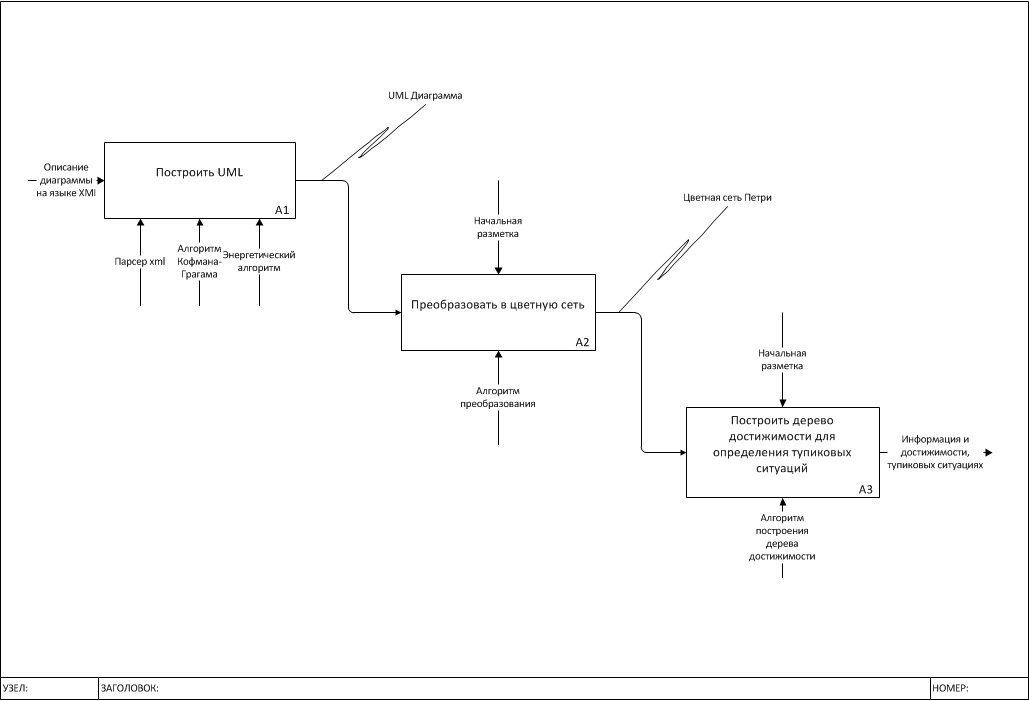
\includegraphics[width=\textwidth]{include/IDEF0.png}
	\end{center}
	\caption{Общий процесс функционирования.}
	\label{fig:fig7}
\end{figure}

Диаграмма деятельности представляет собой граф, вершины которого обозначают действия, а дуги ~--- переходы от одного действия к другому. Способы преобразования UML-диаграмм в простую сеть Петри широко известны, но для преобразования в раскрашенную сеть одних данных диаграммы не хватает: для раскрашенной сети необходимо сформировать множество типов и определить раскраски вершин (т.е. определить тип входных переменных). Процесс преобразования в раскрашенную сеть Петри представлен на рис. \ref{fig:fig8}.

\begin{figure}
	\begin{center}
		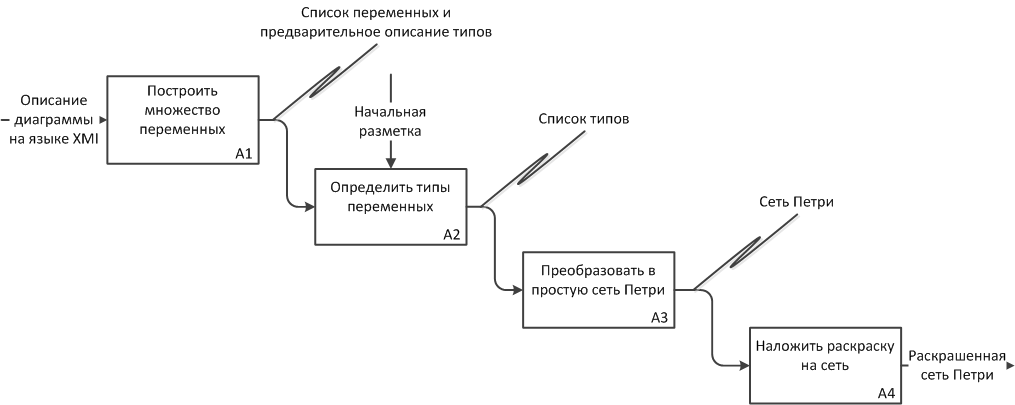
\includegraphics[width=\textwidth]{include/IDEF0ColoredPetri.png}
	\end{center}
	\caption{Процесс преобразования UML диаграммы деятельности в раскрашенную сеть Петри.}
	\label{fig:fig8}
\end{figure}

\section{Рисование бесконтурных графов}

Любую диаграмму деятельности можно свести к планарному графу, а значит и сеть Петри, построенную по этой диаграмме можно отобразить как планарный граф. Будем предполагать, что исходный бесконтурный граф является так называемым \textit{st-графом}, т.е. в нем имеется только одна начальная вершина, обозначаемая через \textit{s}, и одна конечная, обозначаемая через \textit{t}.

Аналитический алгоритм планарного представления графа описывает последовательность различных преобразований, приводящую к построению укладки. \cite{Battista} Краткий план работы алгоритма таков:
\begin{enumerate}
\item[1.] Построение ассоциированного орграфа G*.
\item[2.] Топологическая сортировка G и G*.
\item[3.] Мозаичное представление графа G.
\item[4.] Полилинейное изображение графа G, основанное на мозаичном представлении и информации о типах входных и выходных позиций.
\end{enumerate}

Рассмотрим каждый этап работы алгоритма подробнее.

\subsection{Построение ассоциированного орграфа G*}

Пусть G* ~--- планарный \textit{st-граф}, и пусть $ V, E и F $ - множества вершин, ребер и граней графа G, где внешние грани представлены в F двумя элементами $ s* $ и $ t* $, называемыми левой и правой внешней гранью G.
Определим орграф G*, ассоциированный с G, следующим образом:
\begin{itemize}
\item вершинами G* являются элементы из F;
\item для любой дуги $ e \neq (s, t) $ в G, граф G* имеет дугу $ e* = (f, g) $, где $ f $ ~--- левая по отношению к $ e $ грань, а $ g $ ~--- правая.
\end{itemize}

Для построения G* необходимо получить список всех граней графа G. Для данной задачи условимся понимать под гранью простой цикл графа, не содержащий в себе других циклов. Для поиска циклов используем модификацию алгоритма поиска в глубину:
\begin{verbatim}
function findBaseFaces(matrix, index, used[], track[]):
    used[index] = true;
    foreach outgoing vertex : v from vertex[index]:
        if not used[v]:
            track << v
            // Запуск поиска в глубину из текущей вершины.
            findBaseFaces(matrix, v, used, track)
            // Если вершина еще содержится в списке, то удаляем ее оттуда,
            // т.к. она не содержится в цикле.
            if (track.last = v)
                track remove last
        else if (track contains v) and (track.last <> v):
            // Берем вершины из списка пути следования
            // пока не встретится текущая вершина.
            previous = v;
            while v <> k:
                k << track
                faces << (previous, k)
                used[k] = not used[k]
                previous = k

            // Удаляем первую дугу цикла из графа, тем самым нарушая цикл,
            // и запускаем поиск из текущей вершины заново.
            (u, v) << faces.last
            matrix[u, v] = matrix[v, u] = 0
            continue cycle from begining
\end{verbatim}

Для поиска циклов необходимо преобразовать граф G в неориентированный граф простым симметричным отображением относительно главной диагонали. Алгоритм использует массив used для определения уже просмотренных вершин и список track, содержащий в себе вершины текущей итерации обхода. Если текущая вершина еще не была просмотрена, то запускаем поиск из нее, иначе, если эта вершина уже встречалась и это вершина не является предшественником текущей, мы нашли цикл.

Для нахождения всех вершин, содержащихся в цикле, мы забираем все вершины из списка track на пути до текущей, помечаем их как не пройденные, т.к. они могут содержаться в другом цикле, и добавляем дуги в список faces. После этого удаляем из графа первую дугу цикла. Так как поиск в глубину идет с лева на право, то если эта дуга содержится в другом цикле, то этот цикл уже был найден на предыдущих шагах. 

\begin{figure}
	\begin{minipage}[H]{0.49\linewidth}
		\center{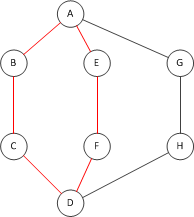
\includegraphics[scale=1]{include/RemoveCycles1.png} \\ Найден цикл (A,B) \rightarrow (B,C) \rightarrow (C,D) \rightarrow (D,F) \rightarrow (F,E) \rightarrow (E,A). \\ Удаляется первое ребро цикла (A,B).}
	\end{minipage}
	\hfill
	\begin{minipage}[H]{0.49\linewidth}
		\center{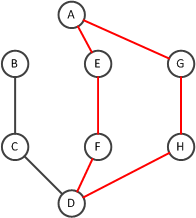
\includegraphics[scale=1]{include/RemoveCycles2.png} \\ Найден цикл (A,E) \rightarrow (E,F) \rightarrow (F,D) \rightarrow (D,H) \rightarrow (H,G) \rightarrow (G,A). \\ Удаляется первое ребро цикла (A,E).}
	\end{minipage}
	\hfill
	\begin{minipage}[H]{0.49\linewidth}
		\center{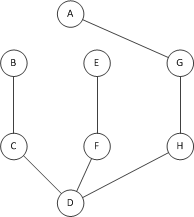
\includegraphics[scale=1]{include/RemoveCycles3.png} \\ Циклов больше нет.}
	\end{minipage}
	\caption{Демонстрация работы алгоритма поиска реберных граней.}
	\label{fig:fig11}
\end{figure}

На основе множества граней графа G необходимо для каждого ребра определить левую и правую грани (рис. \ref{fig:fig12}) и по ним построить граф G*. Для определения ориентации ребер воспользуемся тем, что номера вершин и переходов упорядочены, т.е. дуга $ 1 \rightarrow 2 $ будет раньше, чем дуга $ 1 \rightarrow 3 $. Отсюда следует, что для определения положения граней относительно ребра необходимо определить на правом или левом пути из истока лежит эта грань. Для определения истока необходимо найти на грани вершину, из которой есть только исходящие дуги, но воспользовавшись тем, что вершины упорядочены, можно утверждать, что истоком будет вершина с наименьшим номером. Получаем, что если ребро лежит на левом пути из истока в сток грани, то грань относительно этого ребра правая, иначе ~--- левая.

\begin{figure}
	\begin{minipage}[H]{0.49\linewidth}
		\center{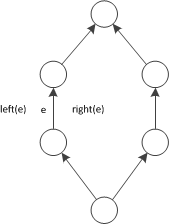
\includegraphics[scale=1]{include/EdgeOrientation.png}}
	\end{minipage}
	\hfill
	\begin{minipage}[H]{0.49\linewidth}
		\center{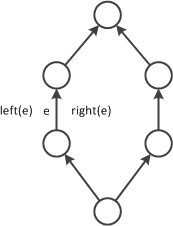
\includegraphics[scale=1]{include/VertexOrientation.png}}
	\end{minipage}
	\caption{Функции \textit{left} и \textit{right} для ориентированного графа.}
	\label{fig:fig12}
\end{figure}

Таким образом, получив для каждого ребра графа G левую и правую грань, выстраиваем матрицу смежности графа G* как переход из левой грани в правую. Матрица смежности G* понадобится в дальнейшем для топологической сортировки уровней G*, таким образом, нет нужды учитывать количество одинаковых дуг из одной грани в другую.

\subsection{Топологическая сортировка сетей}

Топологическая сортировка представляет собой алгоритм упорядочивания вершин бесконтурного ориентированного графа согласно частичному порядку, заданному ребрами орграфа на множестве его вершин. На первом шаге алгоритма мы выбираем все вершины с нулевой полустепенью захода, заносим их в нулевой уровень и исключаем их из графа. В результате, (больше не учитываются строки матрицы, соответствующие обработанным вершинам) полустепени захода остальных вершин уменьшатся. Шаги повторяются пока все вершины не будут просмотрены и распределены по уровням.

На рисунке \ref{fig:fig13} приведена итеративная работа алгоритма.

\begin{figure}
	\begin{minipage}[H]{0.99\linewidth}
		\center{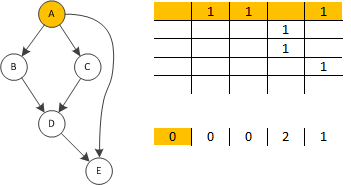
\includegraphics[scale=1]{include/TopologicalSort1.png} \\ Первая итерация. Вершина A не имеет входящих дуг.}
	\end{minipage}
	\vfill
	\begin{minipage}[H]{0.99\linewidth}
		\center{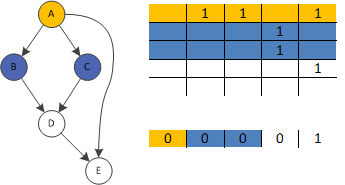
\includegraphics[scale=1]{include/TopologicalSort2.png} \\ Вторая итерация. Вершины B и С не имеют входящих дуг.}
	\end{minipage}
	\vfill
	\begin{minipage}[H]{0.99\linewidth}
		\center{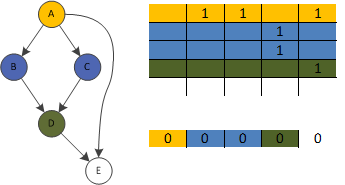
\includegraphics[scale=1]{include/TopologicalSort3.png} \\ Третья итерация. Вершина D не имеет входящих дуг. }
	\end{minipage}	
	\vfill
	\begin{minipage}[H]{0.99\linewidth}
		\center{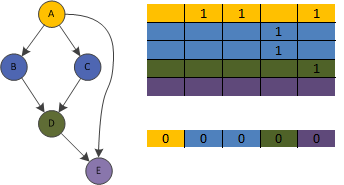
\includegraphics[scale=1]{include/TopologicalSort4.png} \\ Четвертая итерация. Вершина E не имеет входящих дуг. \\ Все вершины просмотрены, окончание работы алгоритма.}
	\end{minipage}
	\caption{Итеративная работа алгоритма топологической сортировки сети.}
	\label{fig:fig13}
\end{figure}

Если граф содержит цикл, то алгоритм на очередном шаге не сможет найти такую вершину, у которой полустепень захода равна нулю, другими словами, нельзя топологически представить цикл, т.к. для него нарушается правило $ X(p) > X(q) \Leftrightarrow (q, p) \epsilon E $.

\subsection{Мозаичное представление графа}

Мозаичное представление $ \Theta $ графа G ~--- это такое отображение каждого объекта $ O $ из $ V \bigcup E \bigcup F $ в плитку $ \Theta(O) $, что справедливы следующие свойства:
\begin{itemize}
\item если $ O_{1} \neq O_{2} $, то нет общих внутренних вершин у $ \Theta(O_{1}) $ и $ \Theta(O_{2}) $;
\item объединение всех плиток $ \Theta(O) $, $ O \epsilon V \bigcup E \bigcup F $ является прямоугольником;
\item $ \Theta(O_{1}) $ и $ \Theta(O_{2}) $ горизонтально инцидентны тогда и только тогда, когда $ O_{1} = left(O_{2}) , O_{1} = right(O_{2}) $ или $ O_{2} = left(O_{1}) , O_{2} = right(O_{1}) $;
\item $ \Theta(O_{1}) $ и $ \Theta(O_{2}) $ вертикально инцидентны тогда и только тогда, когда $ O_{1} = orig(O_{2}) , O_{1} = dest(O_{2}) $ или $ O_{2} = orig(O_{1}) , O_{2} = dest(O_{1}) $;
\end{itemize}

Вершины $ p \epsilon V $ графа G помечаются числами Y(p) таким образом, что Y(s) = 0 и $ Y(p) > Y(q) \leftrightarrow (q, p) \epsilon E $ ~--- дуга G.

Вершины $ p* \epsilon V* $ графа G* помечаются числами X(p*) таким образом, что X(s*) = 0 и $ X(p) > X(q) \leftrightarrow (q, p) \epsilon E* $ ~--- дуга G*.

Для каждой вершины вычисляются координаты горизонтального сегмента \ref{F:F1}:
\begin{equation}
	\begin{cases}
	y = Y(v) \\
	x_{1} = X(left(v)) \\
	x_{2} = X(right(v))
	\end{cases}
\label{F:F1}
\end{equation}

Для каждого ребра графа G вычисляются координаты вертикального сегмента \ref{F:F2}:
\begin{equation}
	\begin{cases}
	y = X(left(e)) \\
	x_{1} = Y(orig(e)) \\
	x_{2} = Y(dest(e))
	\end{cases}
\label{F:F2}
\end{equation}

\begin{figure}
	\begin{center}
		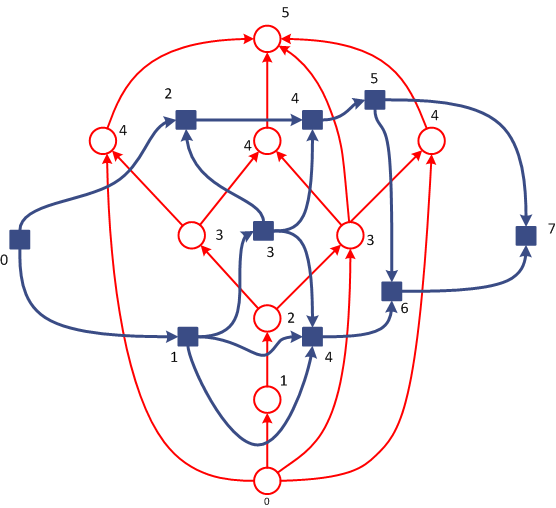
\includegraphics[scale=1]{include/Graph.png}
	\end{center}
	\caption{Планарный \textit{st}-граф G и ассоциированный граф G*.}
	\label{fig:fig14}
\end{figure}

\begin{figure}
	\begin{center}
		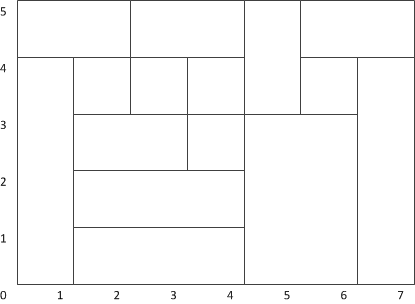
\includegraphics[scale=1]{include/MosaicView.png}
	\end{center}
	\caption{Мозаичное представление графа G.}
	\label{fig:fig15}
\end{figure}

Обзорным представлением Г заданного \textit{st-графа} G называется такое его изображение, в котором каждая его вершина p представлена горизонтальным отрезком Г(p), называемым вершинным отрезком, а каждая дуга (p, q) ~--- вертикальным отрезком Г(p, q), называемым реберным отрезком, таким образом, что справедливы следующие свойства:
\begin{itemize}
\item вершинные отрезки не накладываются друг на друга;
\item реберные отрезки не накладываются друг на друга;
\item реберный отрезок Г(p, q) имеет нижнюю границу, лежащую на Г(p), и верхнюю границу, лежащую на Г(q), и не пересекают ни один другой вершинный отрезок.
\end{itemize}

\subsection{Полилинейное изображение графа G}

Легко конструируется полилинейное изображение планарного \textit{st-графа} G на основе его обзорного представления. Для этого каждая вершина G может быть представлена некоторой точкой соответствующего вершинного отрезка, а каждая дуга (p, q) графа G ломанной, среднее звено которого образовано частью реберного отрезка, изображающего жту дугу (p, q).

Для каждой вершины заменить вершинный отрезок Г(v) на произвольную (среднюю) точку P(v) = (x(v), y(v)) отрезка Г(v).

Для каждого ребра (u, v), если это короткое ребро, т.е. расстояние y(v) - y(u) = 1, заменить реберный отрезок Г(u, v) на отрезок с конечными вершинами P(u), P(v). Иначе, если это ребро длинное, то заменить реберный отрезок Г(u, v) на ломаную линию, соединяющую точки P(u) и P(v) через точки $ (x(U(u, v)), y(u) + 1) $ и $ (x(Г(u, v)), y(u) - 1) $.

\begin{figure}
	\begin{center}
		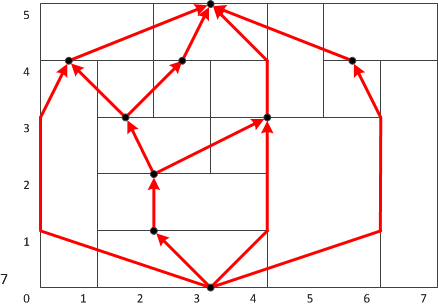
\includegraphics[scale=1]{include/PolylineView.png}
	\end{center}
	\caption{Полилинейное изображение графа G.}
	\label{fig:fig16}
\end{figure}

Наиболее оптимальное размещение точки P(v) ~--- это середина вершинного отрезка Г(v). При этом будет получаться плоское восходящее изображение, имеющее не более 6n - 12 сгибов, а каждое ребро имеет не более двух сгибов. При выборе позиции вершины P(v) в случае стратегии "выбора длинного ребра" можно размещать ее на внешней стороне вершинного отрезка и алгоритм будет строить полилинейное изображение графа в области размера $ O(n^{2}) $ с общим числом вершин $ (10 * n - 31) / 3 $ и не более, чем с двумя сгибами на одном ребре.

\section{Описание UML диаграмм с помощью XMI}

Для описания диаграммы деятельности используется стандарт XMI. Каждая вершина имеет имя, тип и уникальный идентификатор, описанные как атрибуты, и список входных и выходных вершин. Идентификатор используется для связи между вершинами и переходами. Если вершина имеет тип \textit{action}, то она может содержать описание действий, по которым в дальнейшем будет выстраиваться множество переменных.

Каждый переход имеет строго одну исходящую и входящую вершину и может содержать в себе правила защиты перехода (например, для условного перехода \textit{condition}).

Основываясь на описанных правилах, получим структуру описания диаграммы:

\begin{verbatim}
<activity_diagram>
    <states>
        <state id, name, type>
            <incoming transitions>
            <outgoing transition>
            <action>
        </state>
    </states>
    <transitions>
        <transition id>
            <source state>
            <target state>
            <guard>
        </transition>
    </transitions>
<activity_diagram>
\end{verbatim}

\section{Преобразование диаграммы деятельности в раскрашенную сеть Петри}

Наибольшей сложностью в процессе преобразования диаграммы в раскрашенную сеть Петри является формирование самой раскраски сети. Не существует четких правил, по которым можно определить достаточность раскраски, а так же возникает проблема избыточности, при которой сформированная сеть не будет точно моделировать работу диаграммы или не будет работать вовсе из-за невозможности совершения перехода.

Сам алгоритм построения раскрашенной сети Петри можно разделить на четыре этапа:
\begin{enumerate}
\item[1.] Выделение списка переменных для каждой вершины (рис. \ref{fig:fig17}).
\item[2.] Преобразование диаграммы деятельности в простую сеть Петри.
\item[3.] Введение начальной разметки и формирование типов для соответствующих переменных. Предварительное определение множества раскрасок (рис. \ref{fig:fig18}).
\item[4.] Определение максимальной области видимости переменных и формирование результирующей раскраски (рис. \ref{fig:fig19}).
\end{enumerate}

\begin{figure}
	\begin{minipage}[H]{0.49\linewidth}
		\center{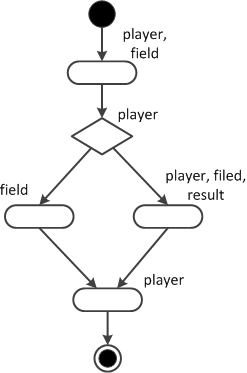
\includegraphics[scale=1]{include/ConvertVariables.png}}
		\caption{Выделение списка переменных.}
		\label{fig:fig17}
	\end{minipage}
	\hfill
	\begin{minipage}[H]{0.49\linewidth}
		\center{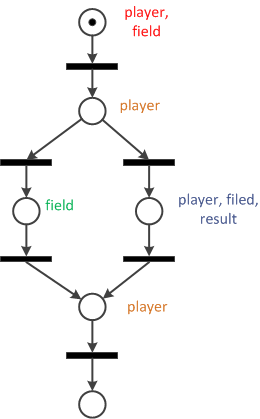
\includegraphics[scale=1]{include/ConvertDiagram.png}}
		\caption{Преобразование в простую сеть Петри и предварительное формирование множества раскрасок.}
		\label{fig:fig18}		
	\end{minipage}
\end{figure}

\begin{figure}
	\begin{minipage}[H]{0.8\linewidth}
		\center{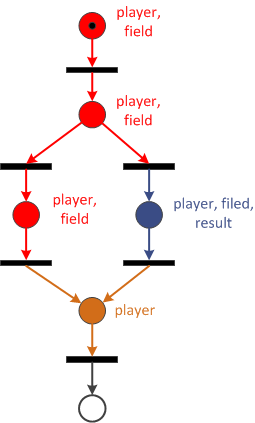
\includegraphics[scale=1]{include/ConvertColoring.png}}
		\caption{Формирование результирующей раскраски.}
		\label{fig:fig19}
	\end{minipage}	
\end{figure}

Исходя из общих правил формирования множества раскрасок, необходимо каждое составное действие разделить на объект, субъект и само действие (\ref{fig:fig9}).

\begin{figure}
	\begin{center}
		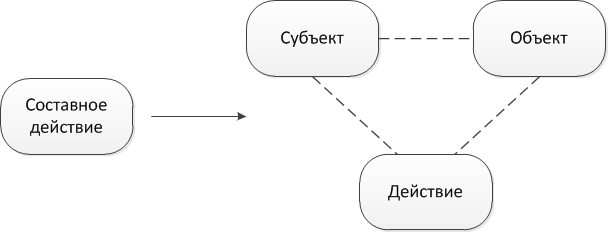
\includegraphics[width=0.6\textwidth]{include/CompositeActivity.png}
	\end{center}
	\caption{Треугольник сложного действия.}
	\label{fig:fig9}
\end{figure}

Сначала выделяются субъект и объект действия. Если на объект действия накладываются условные ограничения (не всегда может быть доступен, например, канал передачи данных, свободный блок оперативной памяти и т.п.), его необходимо отделить от субъекта действия, так как в сети Петри он будет обеспечивать второе условие для срабатывания перехода действия. Субъект и объект действия в общем случае связаны правилом, в соответствии с которым это действие происходит. \cite{Korotkov} 

\subsection{Получение списка переменных}

На первом этапе построение раскрашенной сети необходимо рассмотреть множество переменных, описывающих работу диаграммы. Условимся, что если переменные (в любой части описания переменной) имеют одинаковые имена, то они имеют и одинаковые типы.

На основе этого мы можем построить предварительное описание типов. Предположим, что на диаграмме имеются три блока действия:
\begin{verbatim}
player.cell = field.cell;
player.resource = player.resoure + field.resource;
player.resource = player.resoure - resource.
\end{verbatim}

По этому описанию можно заключить, что в системе фигурируют три переменные: player, field и resource, причем первые две имеют составной тип. Так же получаем то, что типы player и resource имет одинаковое описание типов: $ { cell, resource } $, причем тип всех переменных resource одинаковый. Таким образом, после первого этапа анализа получаем:

\begin{verbatim}
player : struct { cell, resource }
field : struct { cell, resource }
resource : simple type
\end{verbatim}

\subsection{Введение начальной разметки}

На втором этапе пользователю предлагается задать входные данные для диаграммы, основываясь переменных, выделенных на пером этапе. Основываясь на этих значениях, можно построить заключение о типах переменных. Остановим выбор на трех простейших типах: \textit{integer}, \textit{boolean}, \textit{string}, из которых можно образовывать кортежи и сложные структуры.

Для примера, приведенного на первом этапе, построим множество типов:

\begin{verbatim}
player : [ ((1, 1), 0) ]
field : [ ((1, 2), 2); ((1, 3), 1); ((2, 1), 1); ... ]
resource : 1
\end{verbatim}

Учитывая предварительное описание типов, получаем

\begin{verbatim}
player : struct { cell : (int * int), resource : int }
field : struct { cell : (int * int), resource : int }
resource : int
\end{verbatim}

Раскраска характеризуется кортежом типов. Так как каждая позиция содержит список переменных, на этом этапе можно сформировать предварительное множество раскрасок.

При введении начальной разметки значения переменных присваиваются первому вхождению этой переменной на пути из начальной вершины, а для остальных вершин, содержащих эту переменную, значения будут передаваться при функционировании системы с помощью фишек.

\subsection{Преобразование в простую сеть Петри}

Диаграмма деятельности во многом подобна сетям Петри. Но в сетях Петри действия моделируются переходами, а на диаграмме деятельности узлами. Кроме того, если в диаграмме деятельности движение фишки необходимо приостановить, то это делается между узлами на дугах, а не внутри блока. Таким образом, правильный перевод в сеть Петри заменяет узлы на переходы, а дуги на позиции. Узлы диаграммы представляются по-разному, в зависимости от типа (\ref{fig:fig10}):

\begin{figure}
	\begin{minipage}[h]{0.5\linewidth}
		\center{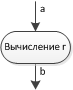
\includegraphics[scale=1]{include/Activity.png}}
	\end{minipage}
	\hfill
	\begin{minipage}[h]{0.4\linewidth}
		\center{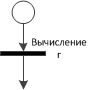
\includegraphics[scale=1]{include/ActivityPetri.png}}
	\end{minipage}
	\hfill
	\begin{minipage}[h]{1\linewidth}
		\begin{tabular}{ p{0.5\linewidth} p{0.5\linewidth} }
			\centering 1. & \centering 2. \\
		\end{tabular}
	\end{minipage}
	\hfill	
	
	\begin{minipage}[h]{0.5\linewidth}
		\center{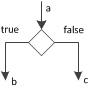
\includegraphics[scale=1]{include/Condition.png}}
	\end{minipage}
	\hfill	
	\begin{minipage}[h]{0.4\linewidth}
		\center{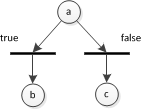
\includegraphics[scale=1]{include/ConditionPetri.png}}
	\end{minipage}
	\hfill
	\begin{minipage}[h]{1\linewidth}
		\begin{tabular}{ p{0.5\linewidth} p{0.5\linewidth} }
			\centering 3. & \centering 4. \\
		\end{tabular}
	\end{minipage}
	\hfill		
	
	\begin{minipage}[h]{0.5\linewidth}
		\center{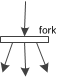
\includegraphics[scale=1]{include/Fork.png}}
	\end{minipage}
	\hfill	
	\begin{minipage}[h]{0.4\linewidth}
		\center{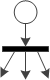
\includegraphics[scale=1]{include/ForkPetri.png}}
	\end{minipage}
	\hfill	
	\begin{minipage}[h]{1\linewidth}
		\begin{tabular}{ p{0.5\linewidth} p{0.5\linewidth} }
			\centering 5. & \centering 6. \\
		\end{tabular}
	\end{minipage}
	\hfill		
	
	\begin{minipage}[h]{0.5\linewidth}
		\center{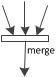
\includegraphics[scale=1]{include/Merge.png}}
	\end{minipage}
	\hfill
	\begin{minipage}[h]{0.4\linewidth}
		\center{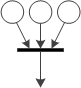
\includegraphics[scale=1]{include/MergePetri.png}}
	\end{minipage}
	\begin{minipage}[h]{1\linewidth}
		\begin{tabular}{ p{0.5\linewidth} p{0.5\linewidth} }
			\centering 7. & \centering 8. \\
		\end{tabular}
	\end{minipage}
	\hfill		
	
	\caption{Преобразование узлов диаграммы деятельности в сеть Петри.  деятельность; 3,4 условие; 5,6 ветвление; 7,8 синхронизация.}
	\label{fig:fig10}
\end{figure}

Условия для принятия решения в сетях Петри задаются как свойства соответствующих переходов. Позиция, предшествующая ветвлению, имеет два выхода, и маркер позиции перейдет через тот переход, условию которого удовлетворяет его значение. Стоит отметить потенциальную возможность ошибок, предупреждение которых целесообразно рассматривать как одно из формальных правил.
\begin{itemize}
\item Если для переходов ветвления не заданы условия их срабатывания, возникает неопределенность, в какую ветку перейдет маркер.
\item В случае если ни одно из условий не является истинным, переход становится недоступным ~--- маркер остается в своей позиции.
\end{itemize}

\subsection{Наложение раскраски}

На последнем этапе необходимо получить результирующую раскраску сети. На втором этапе была введена предварительная раскраска сети, основанная только на множестве переменных, принадлежащих вершине.

Для каждой переменной необходимо найти максимальную область ее видимости ~--- т.е. все возможные пути из вершины, где она встретилась в первый раз, до вершины, после которой она больше не содержится во множестве используемых переменных.

Основываясь на этом, мы расширяем список используемых переменных вершины и меняем ее раскраску.

\section{Обратная польская запись}

При переходе от диаграммы деятельности к раскрашенной сети Петри мы выделяем список переменных, на основе которых строится раскраска. При функционировании моделируемой системы переход сети может менять раскраску используемых фишек, а значит, и производить над ними вычисления. В связи с этим встает задача разбора и вычисления математических выражений. Как правило, арифметические выражения удобно преобразовывать в обратную польскую запись, чтобы избавиться от скобок, содержащихся в выражении. Выражения, преобразованные в польскую запись, можно вычислять последовательно, слева направо.

Отличительной особенностью обратной польской нотации является то, что все аргументы (или операнды) расположены перед знаком операции. В общем виде запись выглядит следующим образом:
\begin{itemize}
\item Запись набора операций состоит из последовательности операндов и знаков операций. Операнды в выражении при письменной записи разделяются пробелами.
\item Выражение читается слева направо. Когда в выражении встречается знак операции, выполняется соответствующая операция над двумя последними встретившимися перед ним операндами в порядке их записи. Результат операции заменяет в выражении последовательность её операндов и её знак, после чего выражение вычисляется дальше по тому же правилу.
\item Результатом вычисления выражения становится результат последней вычисленной операции.
\end{itemize}

Автоматизация вычисления выражений в обратной польской нотации основана на использовании стека. Алгоритм вычисления для стековой машины элементарен:
\begin{enumerate}
\item[1.] Обработка входного символа.
\begin{enumerate}
\item[1.1.] Если на вход подан операнд, он помещается на вершину стека.
\item[1.2.] Если на вход подан знак операции, то соответствующая операция выполняется над требуемым количеством значений, извлечённых из стека, взятых в порядке добавления. Результат выполненной операции кладётся на вершину стека.
\end{enumerate}
\item[2.] Если входной набор символов обработан не полностью, перейти к шагу 1.
\item[3.] После полной обработки входного набора символов результат вычисления выражения лежит на вершине стека.
\end{enumerate}

Реализация стековой машины, как программная, так и аппаратная, чрезвычайно проста и может быть очень эффективной. Обратная польская запись совершенно унифицирована ~--- она принципиально одинаково записывает унарные, бинарные, тернарные и любые другие операции, а также обращения к функциям, что позволяет не усложнять конструкцию вычислительных устройств при расширении набора поддерживаемых операций.

Существует несколько алгоритмов для превращения инфиксных формул в обратную польскую запись. Наиболее распространен переработанный алгоритм, идея которого предложена Э.В. Дейкстрой.

Для хранения переменных используется стек типа char.

Рассматриваем поочередно каждый символ:
\begin{enumerate}
\item[1.] Если этот символ - число (или переменная), то просто помещаем его в выходную строку.
\item[2.] Если символ ~--- знак бинарной операции (+, -, *, /), то проверяем приоритет данной операции. Получив один из этих символов, мы должны проверить стек:
\begin{enumerate}
\item[2.1.] Если стек все еще пуст, или находящиеся в нем символы имеют меньший приоритет, чем приоритет текущего символа, то помещаем текущий символ в стек.
\item[2.2.] Если символ, находящийся на вершине стека имеет приоритет, больший или равный приоритету текущего символа, то извлекаем символы из стека в выходную строку до тех пор, пока выполняется это условие; затем переходим к пункту 2.1.
\end{enumerate}
\item[3.] Если текущий символ - открывающая скобка, то помещаем ее в стек.
\item[4.] Если текущий символ - закрывающая скобка, то извлекаем символы из стека в выходную строку до тех пор, пока не встретим в стеке открывающую скобку, которую следует просто уничтожить. Закрывающая скобка также уничтожается.
\end{enumerate}

Если вся входная строка разобрана, а в стеке еще остаются знаки операций, извлекаем их из стека в выходную строку.

\section{Алгоритм построения дерева достижимости}

Алгоритм начинает свою работу с определения начальной разметки. До тех пор, пока имеются граничные вершины, они обрабатываются алгоритмом.

Пусть x – граничная вершина, которую необходимо обработать, и с которой связана разметка $ \mu(x) $.
\begin{enumerate}
\item Если в дереве имеется другая вершина y, не являющаяся граничной, и с ней связана разметка $ \mu(y) = \mu(x) $, то вершина x дублируется. 
\item Если для разметки $ \mu(x) $ ни один из переходов неразрешим, т.е. $ \mu(x) $ тупиковая разметка, то x терминальная вершина.
\item Для любого перехода $ t_{j} $, из множества T разрешенного в разметке $ \mu(x) $, создать новую вершину z дерева достижимости. Разметка $ \mu(z) $, связанная с этой вершиной, определяется для каждой позиции $ p_{i} $ следующим образом:
\begin{enumerate}
\item если $ \mu(x)_{i} = \omega, то \mu(z)_{i} = \omega $;
\item если на пути от корневой вершины к x существует вершина y такая, что $ \mu(y)\rightarrow^{t_{j}} \mu(x), \mu(y) < \mu(x) и \mu(y)_{i} < \mu(x)_{i} $, то $ \mu(z)_{i} = \omega $;
\item в противном случае $ \mu(z)_{i} = \mu(x)_{i} $.
\end{enumerate}

\end{enumerate}

Дуга, помеченная $ t_{j} $, направлена от вершины х к вершине z. Вершина x переопределяется как внутренняя, вершина z становится граничной. Когда все вершины дерева становятся терминальными, дублирующими или внутренними, алгоритм останавливается. Из алгоритма построения дерева достижимости следуют следующие выводы:
\begin{itemize}
\item сеть ограничена тогда и только тогда, когда символ $ \omega $ отсутствует в дереве;
\item сеть безопасна, если число фишек в каждой позиции не превышает 1;
\item сеть живая, если в дереве отсутствуют циклы и тупики.
\end{itemize}

\label{cha:design}

\chapter{Технологический раздел}

\section{Выбор и обоснование языка программирования}

Для разработки программного комплекса был выбран язык C++ и среда разработки Qt 4.8. Данная среда является кроссплатформеной и обладает огромной библиотекой классов, что существенно упрощает разработку. Для перенесения программы на другую операционную систему требуется лишь ее перекомпиляция. Язык C++ является мощнейшим инструментом разработки: он имеет строгую типизацию и объектно-ориентирован, обеспечивает возможность быстрой разработки приложений, но при этом сохраняет выразительность и элегантность.

\section{Структура программного комплекса}

Внутреннее строение системы имеет модульную структуру. Каждый модуль отвечает за определенные функции системы. Все модули и классы, реализованные в нем, можно разделить на два типа:
\begin{itemize}
\item классы, реализующие интерфейс программы;
\item классы,отвечающие за логику работы программы.
\end{itemize}

Было принято решение не выделять отдельной сущностью менеджера, т.к. система имеет практически линейный сценрий и к ней не предъявляются требования по сохранению собственного состояния. Вся нагрузка по взаимодействию классов ложится на класс главной формы. Стоит отметить, что реакция системы на неверные входные данные реализована в виде негативного результата функции, т.к. механизм исключений \textit{try} ... \textit{catch} не имеет должной поддержки в Qt из-за особенностей реализации.

На вход системе поступает XMI-файл, содержащий описание диаграммы. Разбор и построение списка состояний и переходов диаграммы производится в методе \textit{parse} класса \textit{XMLEngine} . Исходя из особенностей структуры XMI разбор файла производится вручную. Для этого, перед основной функцией разбора вызывается метод \textit{validate} класса \textit{XMLValidator}, который проверяет соответствие файла имеющейся xml-схеме. В ходе разбора сначала заполняется список состояний диаграммы states, а потом, основываясь на этом списке строиться список переходов transitions. Каждое состояние имеет свой уникальный id, по которому происходит связывание текущего перехода transition с исходной и целевой вершиной.

В случае удачного разбора файла происходит отображение диаграммы. Для большей гибкости приложения, само рисование диаграмы вынесено в отдельный класс и используется паттер посетитель для ее отображения. Парадигма ядра графического движка Qt основана на представлении отдельных примитивов как объектов и дальнейшим их позиционировании на плоскости.

Каждый потомок абстрактного класса \textit{State} имеет переопределенный метод \textit{diagramItem()}, который создает соответствующий класс, наследуемый от абстрактного \textit{QGraphicsItem}, и отвечающий за отображение этого типа элемента диаграммы.

Диаграмма классов представленна на рисунке \ref{fig:fig1}.

%\begin{figure}
%	\begin{center}
%		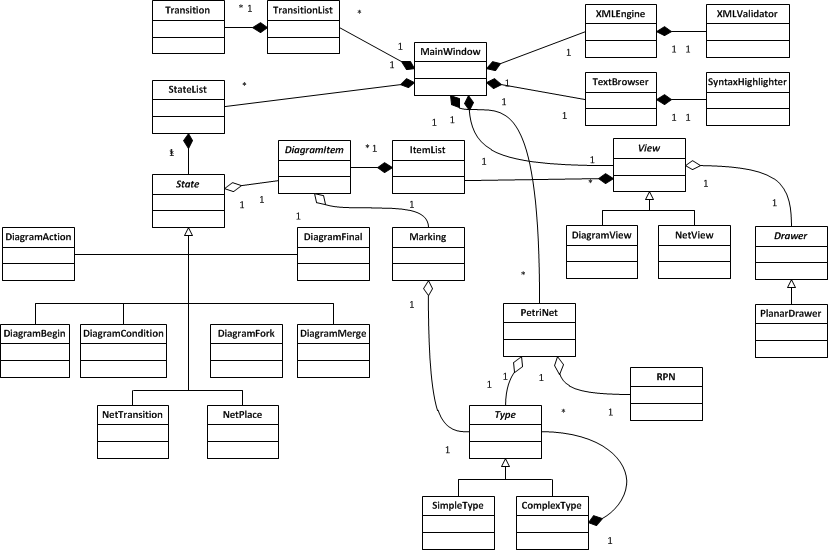
\includegraphics[scale=1]{include/ClassDiagram.png}
%	\end{center}
%	\caption{Диаграмма классов системы}
%	\label{fig:fig1}
%\end{figure}

\section{Алгоритм работы системы}

\subsection{Построение списка переменных}

Для преобразования в раскрашенную сеть Петри необходимо иметь информацию о переменных, используемых диаграммой. Переменные могут фигурировать в диаграмме в блоках действий или как спусковые функции переходов. Для разобра переменных будем использовать алгоритм поиска в глубину. Структура данных для описания типов приведена на рисунке \ref{fig:fig2}.

\begin{figure}
	\begin{center}
		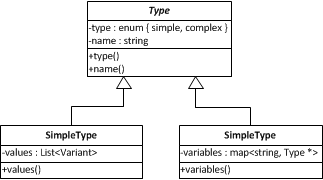
\includegraphics[scale=1]{include/Type.png}
	\end{center}
	\caption{Структура классов описание типов переменных}
	\label{fig:fig2}
\end{figure}

Все переменные можно разделить условно на два типа: простые и составные (структурные). Для простых переменных используется список сериализованных данных \textit{list<variant>}. Структурный тип имеет именнованный список переменных \textit{map<string, type *>}.	

\subsection{Преобразование в простую сеть Петри}

Условимся, что элементы преобразуются позиции и переходы. Позиции соединены с переходами, но они не имеют входных дуг, а переходы выходных. Исключения составляют начальное и конечное состояние. Так как начальное состояние имеет только одну выходную дугу, мы можем его вообще не учитывать, а выходной переход преобразуется только в соотвествующую позицию. Так как ограничения переходов могут накладываться только на блок условного перехода, при преобразовании условие преобразуется в спусковую функцию внутренней дуги между позицией и переходом.
Алгоритм преобразования состоит из двух частей:
\begin{itemize}
\item преобразование каждого элемента диаграммы в сооствествующий набор позиций и переходов сети;
\item связывание преобразовыванных элементов друг с другом.
\end{itemize}

Позиции и переходы являются наследниками абстрактного класса \textit{State}, а значит для их идентефикации используется поле \textit{id}. Для каждой позиции идентефикатор формируется как \textit{id} преобразоываемого элемента, метка \textit{place} и порядковый номер, если позиций больше одной. Аналогично для переходов. Из-за этого нарушается четкая взаимосвязь между состояниями и переходами сети, т.е. после первого этапа преобразования нельзя четко сказать какая дуга из  перехода в позицию будет соотвествовать дуге в исходном описании. Необходимо реализовать связь элементов сети, производя поиск незанятых позиций и переходов.
\begin{lstlisting}[style=pseudocode,caption={Алгоритм преобразования в простую сеть Петри}]
List<State *> queue
State * state = states.find(begin_state)
queue.append(state)

while !queue.empty():
	State * state = queue.takeFirst()
	if !netStates->find(state->id()):
		convertState(state)

	foreach transition in state.outgoing:
		if !netStates->find(target->id()):
			queue.append(target)
			convertState(target)

		if state->type() != begin_state:
			State * transition, * place;
			List<State *> transitions = netStates->find(state->id() + "transition")
			if state->type() = condition_state:
				transition = findFreeTransition(transitions)
			else
				transition = transitions.first()

			List<State *> places = netStates->find(target->id() +  "place");
			if target->type() == merge_state:
				place = findFreePlace(places)
			else
				place = places.first()

			Transition * tr = new Transition(state->id() + "-" + target->id())
\end{lstlisting}

\subsection{Формирование множества активных переходов}

В процессе моделирования на каждом шаге возникает задача поиска множества активных переходов. Для решения этой задачи можно последовать двумя путями:

\begin{itemize}
\item поиск всех переходов и выделение списка активных переходов;
\item поиск всех позиций, содержащих фишки, и на основании этого построение списка возможных переходов.
\end{itemize}

Так как каждая позиция может иметь несколько исходящих переходов, а каждый переход может иметь несколько входных позиций, задача определения множества активных переходов в общем случае сводится к полному перебору. С учетом специфики преобразования диаграммы, получаем, что из одной позиции может быть несколько переходов только в случае условного перехода и все исходящие переходы для этой позиции имеют лишь одну входящую дугу. Переход может иметь несколько входных позиций только в случае слияния, а значит все позиции имеют лишь одну исходящую дугу. Для всех остальных случаев каждый переход имеет лишь одну входную дугу, а каждая позиция лишь одну исходящую.

Основываясь на этом, сформулируем алгоритм формирования множества активных переходов:
\begin{lstlisting}[style=pseudocode,caption={Алгоритм формирования множества активных переходов}]
List<Place *> list, places = states->find(place)
MultiMap<Place *, Transition *> activeTransitions
foreach place in places:
	if place->marking > 0:
		list.append(place)
		
foreach transition in place->outgoing:
	bool flag = true
	foreach place in transition->incoming:
		if place->marking = 0:
			flag = false
	if flag:
		activeTransitions.insert(place, transition)
\end{lstlisting}

\section{Анализ работоспособности программного комплекса}

\label{cha:implementation}

% \chapter{Экспериментальный раздел}

\section{Исследование появления блокировок}

Основной задачей исследования сетей Петри является выявление недоступных состояний и блокировок. Выявим причины, по которым они могут возникнуть в диаграммах деятельности. В процессе исследования представим диаграмму деятельности в виде простой и раскрашенной сети Петри и сравним результаты.

В диаграммах деятельности блокировки могут возникать по причине:
\begin{itemize}
\item неверной структуры диаграммы;
\item невозможности перехода из-за невыполнения логического условия спусковой функции.
\end{itemize}

\subsection{Простая сеть Петри}

Так как простые сети Петри могут моделировать лишь поток выполнения, для них возможно выявления лишь структурных несоответствий диаграммы.

Блокировки в сетях Петри могут быть вызваны лишь ситуацией, когда переходу принадлежит два и более места, но не все места имеют фишки. Применительно к диаграмме деятельности, только блок ожидания завершения параллельного процесса может иметь больше одной входной дуги во внутреннем переходе. Таким образом, для получения блокировки внутри блоков многопоточной обработки должен находиться условный переход (рис. \ref{fig:fig22}, \ref{fig:fig23}).

\begin{figure}
	\begin{minipage}[H]{0.49\linewidth}
		\center{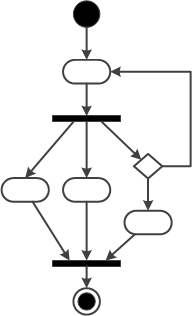
\includegraphics[scale=1]{include/BlockedDiagram1.png}}
	\end{minipage}
	\hfill
	\begin{minipage}[H]{0.49\linewidth}
		\center{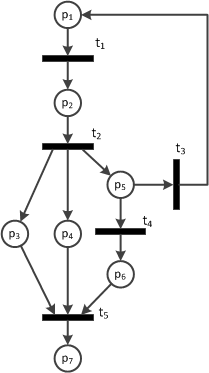
\includegraphics[scale=1]{include/BlockedNet1.png}}
	\end{minipage}
	\caption{Блокировка из-за выхода за пределы блоков.}
	\label{fig:fig22}
\end{figure}

\begin{figure}
	\begin{minipage}[H]{0.49\linewidth}
		\center{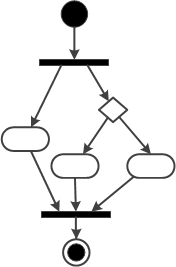
\includegraphics[scale=1]{include/BlockedDiagram2.png}}
	\end{minipage}
	\hfill
	\begin{minipage}[H]{0.49\linewidth}
		\center{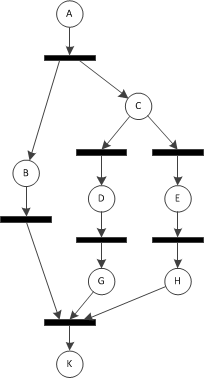
\includegraphics[scale=1]{include/BlockedNet2.png}}
	\end{minipage}
	\caption{Блокировка из-за неверной структуры внутреннего условия.}	
	\label{fig:fig23}	
\end{figure}

Ситуация блокировки, изображенная на рисунке \ref{fig:fig22} искусственная, т.к. по логике выход за пределы параллельных процессов невозможен. Так же, при моделировании такой ситуации получается, что метки C и D являются небезопасными, и в них будет происходить бесконечное накопление фишек.

Ситуация, изображенная на рисунке \ref{fig:fig23} возможна и в результате в системе возникает блокировка, т.к. переход никогда не сработает. Для избежания такой ситуации используется введение дополнительной вершины, из которой будет единственная дуга в блок синхронизации (рис. \ref{fig:fig24}).

\begin{figure}
	\begin{minipage}[H]{0.49\linewidth}
		\center{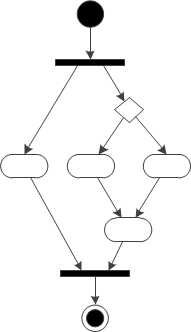
\includegraphics[scale=1]{include/CorrectDiagram.png}}
	\end{minipage}
	\hfill
	\begin{minipage}[H]{0.49\linewidth}
		\center{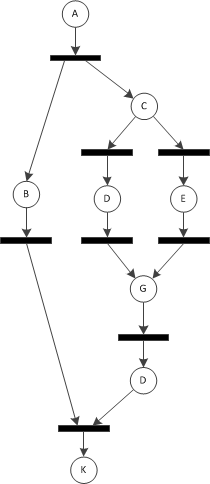
\includegraphics[scale=1]{include/CorrectNet.png}}
	\end{minipage}
	\caption{Корректная структура внутреннего условия.}	
	\label{fig:fig24}	
\end{figure}

\subsection{Раскрашенная сеть Петри}

Диаграмма деятельности имеет практически линейную структуру, за исключением вершины условного перехода, которая при преобразовании в простую сеть будет давать два возможных пути выполнения, т.к. переходы имеют равный приоритет и в простой сети срабатывание перехода определяется лишь наличием фишки в позиции. При наличии некоторого цикла в диаграмме, анализ с помощью простой сети Петри выдаст лишь его наличие.

Моделирование работы диаграммы деятельности с помощью раскрашенных сетей Петри приводит к тому, что пути процесса выполнения будут иметь вид линейную структуру, а не древовидную. Блокировка в сети может быть вызвана не только отсутствием фишки в позиции, но и не срабатыванием спусковой функции из-за невыполнения логического условия.

По этой причине, раскрашенная сеть Петри не всегда способна выявить некорректную структуру диаграммы, т.к. при конкретной начальной разметке, для которой построена сеть, не все переходы будут активны.

\section{Исследование корректности построения раскраски сети}

Предложенный метод формирования раскраски сети на основе определения максимальной видимости переменных в ходе исследования работоспособности метода дал хорошие результаты, но при этом были выявлены ограничения, связанные со структурой преобразуемой диаграммы.

Если в диаграмме имеется хотя бы один цикл, то при наложении раскраски возникает вопрос об определении области видимости переменных. В связи с этим получается два подхода:
\begin{itemize}
\item[1.] определять раскраску всех элементов цикла как кортеж переменных наибольшей мощности (рис. \ref{fig:fig25});
\item[2.] определять раскраску не учитывая обратную дугу цикла (рис. \ref{fig:fig26}).
\end{itemize}

Так как фишка хранит в себе набор переменных, сопоставленных ее цвету, то при реализации первого подхода на переходах внутри цикла будут меняться лишь значение переменных. Такой подход будет вести к некорректному моделированию работы, т.к. если какая либо позиция в цикле содержит несколько фишек, то в процессе моделирования будет использована лишь одна из них, и весь процесс работы будет привязан лишь к значениям переменных.

При реализации второго подхода в сети может случиться блокировка, т.к. фишка из раскраски меньшей мощности будет переходить к более мощной раскраске в позиции не содержащей фишек новой раскраски. Другими словами, при моделировании работы диаграммы на рисунке \ref{fig:fig26} не сможет сработать переход $ t_{6} $ даже если будет выполнено логическое условие, ограничивающее этот переход, т.к. мощность раскраски позиции $ p_{6} $, содержащей фишку, меньше мощности позиции $ p_{2} $.

\begin{figure}
	\begin{minipage}[H]{0.49\linewidth}
		\center{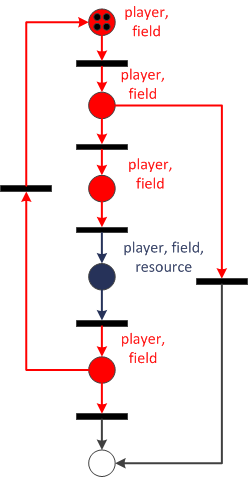
\includegraphics[scale=1]{include/ResearchWithCycle.png}}
		\caption{Сеть с раскраской, наложенной с учетом циклов.}
		\label{fig:fig25}
	\end{minipage}
	\hfill
	\begin{minipage}[H]{0.49\linewidth}
		\center{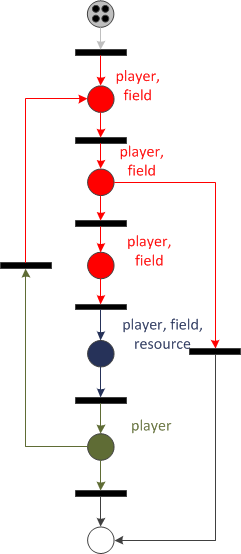
\includegraphics[scale=1]{include/ResearchWithoutCycle.png}}
		\caption{Сеть с наложением раскраски без учета циклов.}
		\label{fig:fig26}
	\end{minipage}
\end{figure}

С учетом вышесказанного было принято решение использовать первый подход, но при нахождении в позиции с ненулевой разметкой заменять фишку, содержащуюся в маркере на новую. Это решение позволяет избежать некорректности работы модели, т.к. в процессе будут использоваться все фишки сети.

\section{Сравнение скорости работы простой и раскрашенной сети Петри}

Проведем сравнение времени работы и затраченных ресурсов для моделирование работы диаграммы деятельности, представленной простой и раскрашенной сетью Петри.

В сравнении времени моделирования учитывалось только время преобразования диаграммы деятельности в сеть и проведение анализа. Результаты сравнения показаны в таблице \ref{tab:table1} и рисунке \ref{fig:fig30}.

\begin{table}
	\caption{Сравнение времени моделирования.}
	\begin{tabular}{|l|c|c|c|}
	\hline
	& 8 состояний & 15 состояний & 25 состояний \\
	\hline
	Простая сеть Петри & 0.012 сек. & 0.015 сек. &  0.020 сек. \\
	\hline
	Раскрашенная сеть Петри & 0.42 сек. & 0.67 сек. &  0.114 сек. \\
	\hline
	\end{tabular}
	\label{tab:table1}
\end{table}

\begin{figure}
	\centering
	\begin{tikzpicture}
		\begin{axis}[width=\textwidth, height=8cm, grid=major, xmin=8, ymin=0,  xlabel=Количество состояний, ylabel=Время моедлирования (мс), no markers]
		\addplot+[smooth] coordinates
		{ (8, 12) (12, 14) (15, 15) (20, 18) (25, 20) (28, 23) };
		\addlegendentry{Простая сеть}
		\addplot+[smooth] coordinates
		{ (8, 45) (12, 56) (15, 67) (20, 89) (25, 113) (28, 143) };
		\addlegendentry{Раскрашенная сеть}
		\end{axis}
	\end{tikzpicture}
	\caption{Сравнение времени моделирования простой и раскрашенной сети.}
	\label{fig:fig30}
\end{figure}

В результате исследования мы получили, что время, затраченное для моделирования раскрашенной сеть Петри значительно больше. Это объясняется тем, что на этапе преобразования диаграммы помимо самого преобразования в сеть Петри происходит так же анализ множества используемых переменных и построение раскраски. Так же во время моделирования для раскрашенной сети на каждом переходе происходит вычисление новых значений переменных, а для каждой дуги из позиции в переход вычисляется спусковая функция.

Для подсчета затраченных ресурсов использовался профилировщик кода VTune. Профилировщик запускал моделирующую программу и по окончанию моделирования выводился список затраченных ресурсов для каждого объекта программы.

\begin{table}
	\caption{Сравнение затраченных ресурсов.}
	\begin{tabular}{|l|c|c|c|}
	\hline
	& 8 состояний & 15 состояний & 25 состояний \\
	\hline
	Простая сеть Петри & 250KB & 340KB & 585KB \\
	\hline
	Раскрашенная сеть Петри & 345KB & 420KB & 730KB \\
	\hline
	\end{tabular}
	\label{tab:table2}
\end{table}

\begin{figure}
	\centering
	\begin{tikzpicture}
		\begin{axis}[width=\textwidth, height=8cm, grid=major, xmin=8, ymin=0,  xlabel=Количество состояний, ylabel=Количество ресурсов, no markers]
		\addplot+[smooth] coordinates
		{ (8, 250) (12, 310) (15, 340) (20, 475) (25, 585) (28, 612) };
		\addlegendentry{Простая сеть}
		\addplot+[smooth] coordinates
		{ (8, 345) (12, 390) (15, 420) (20, 655) (25, 730) (28, 795) };
		\addlegendentry{Раскрашенная сеть}
		\end{axis}
	\end{tikzpicture}
	\caption{Сравнение затраченных ресурсов для простой и раскрашенной сети.}
	\label{fig:fig30}
\end{figure}

В результате исследования было выявлено, что моделирование диаграммы деятельности в виде простой и раскрашенной сети Пери требует приблизительно одинаковое количество ресурсов. Небольшая разница объясняется тем, что в раскрашенной сети для каждой позиции хранится список используемых переменных и цвет, а в переходах и на внутренних дугах содержится выражения.

\label{cha:research}



\backmatter

% \Conclusion

В рамках данно проекта был разработан и реализован метод преобразования диаграммы деятельности в раскрашенную сеть Петри, позволяющий выявить блокировки и недостижимые состояния. В результате работы над проектом были проделаны следующие этапы:
\begin{enumerate}
\item[1.] проведена классификация существующих методов анализа диаграмм деятельности;
\item[2.] реализован алгоритм отображения диаграмм деятельности;
\item[3.] разработан метод представления диаграммы деятельности в виде раскрашенной сети Петри;
\end{enumerate}

Было проведено исследование причин появления блокировок в диаграммах деятельности и применимость простой и раскрашенной сетей для задачи их выявления. Так же было проведено исследование подходов к построению раскраски сети и на основе этих результатов было принято решение об улучшении реализации предложенного метода.
\bibliographystyle{gost780u}
\bibliography{rpz}


\end{document}
